\chapter{Valuation of Financial Derivatives}
    \noindent
    This chapter establishes the mathematical framework underpinning the valuation of financial derivatives. Financial derivatives pricing heavily relies on stochastic calculus to model the random evolution of asset prices and derive prices free of arbitrage \cite{hirsa2013introduction}. We consider a continuous-time financial market model over a finite time horizon $T < \infty$, and the uncertainty in the market is modeled by a  probability space.

    \begin{theorem}[Probability Space] \label{thm:probability-space}
         A \textbf{Probability space} is the triple $(\Omega, \mathcal{F}, \mathbb{Q})$, it provides the mathematical structure for defining random processes and modeling the flow of information.
        \begin{itemize}
            \item $\Omega$ is the set of all market states
            \item $\mathcal{F}$ is a sigma-field describing the flow of information over time, represented by a filtration $\mathcal{F}_t$. It contains historical market prices up to time $t$
            \item $\mathbb{Q}$ is the probability measure (often referred to as the risk-neutral measure or real measure $\mathbb{P}$)
        \end{itemize}
    \end{theorem}
    
    \noindent
    The filtration $(\mathcal{F}_t)_{t \in [0,T]}$ formalises this information structure by specifying precisely what is observable at each instant, ruling out any anticipation of future market realisations. Each financial underlying is then modelled as a stochastic process adapted to this filtration, so that its value at time $t$ depends only on information available up to and including $t$. 

     \newpage
    \begin{definition}[Stochastic Process] \label{def:stochastic-process} 
        A \textbf{stochastic process} is a family of random variables $\{X(t)\}_{t \in [0,T]}$ defined on the probability space $(\Omega, \mathcal{F}, \mathbb{Q})$. For each fixed $t \in [0,T]$, the map $X(t, \cdot) : \Omega \to \mathbb{R}$ is a random variable measurable with respect to $\mathcal{F}_t$. For each fixed $\omega \in \Omega$, the map $t \mapsto X(t, \omega)$ is called a \textbf{sample path} or \textbf{realisation} of the process. The process is said to be \textbf{adapted} to the filtration $(\mathcal{F}_t)_{t \in [0,T]}$ if $X(t)$ is $\mathcal{F}_t$-measurable for every $t$, meaning the value of the process at time $t$ depends only on information available up to and including $t$.
    \end{definition}

    \noindent
    In a financial context, the sample paths $t \mapsto X(t, \omega)$ represent possible trajectories of an asset price, interest rate, or exchange rate over the horizon $[0,T]$, with the measure $\mathbb{Q}$ governing the likelihood of each trajectory. The adaptedness condition is economically natural it ensures the model does not anticipate future information, so the value of any process at time $t$ is determined solely by the history of the market up to that point \cite{blyth2014introduction}. Not every adapted process possesses the structure required for no-arbitrage pricing, of particular importance is the martingale, which captures the idea that, under $\mathbb{Q}$, the best prediction of a process's future value is simply its current value.

    \begin{definition}[Martingale] \label{def:martingale}
        A stochastic process $X_t$ is a \textbf{Martingale}  with respect to filtration $\mathscr{F}_t$ under $\mathbb{Q}$ if the best prediction of its future value, conditioned on current information, is simply its current value
        \begin{equation}
            \mathbb{E} \left[ X_t\right] < \infty   
        \end{equation}    
        and, 
        \begin{equation}
            \mathbb{E} \left[ X_t\right | \mathscr{F}_s ] = X_s \quad  \text{with  s < t} 
        \end{equation}
            
    \end{definition}

    \noindent
     The money market account, sometimes referred to as the bank account. Money market account represents a (locally) riskless investment, where profits is accrued continuously at the risk-free rate prevailing in the market at every instant \cite{brigo2001interest}. Sometimes, the money market or bank account can sometimes be referred to as a default-free bond or a zero-coupon bond. It serves as the natural numeraire in risk-neutral pricing and must be distinguished from the zero-coupon bond, which is a tradable instrument promising a unit payment at a fixed maturity date, the money market account, by contrast, has no fixed maturity and rolls forward continuously at the prevailing short rate. We formalise its dynamics below. 

    \begin{definition}[Bank Account]\label{def:bank_account}
    A \textbf{Bank account (Money-market account)}, we define $B_t$ as the value of the risk-free money market account at time $t$. We assume the account evolves  deterministically according to the risk-free short rate $r_t$:   

    \begin{equation}
        dB_t = r_tB_tdt, \quad B_0 = 1
    \end{equation}
    
    \end{definition}
    Where $r_t$ is a positive function of time. As a result, 

    \begin{equation}
        B_t = B_0\text{exp}  \left( \int_{0}^{t} r_s ds\right)
    \end{equation}

    \noindent
    Discounted stock prices are said to be martingales under the risk-neutral probability measure. Martingale is the probabilistic definition of a fair game, where the expected value of a portfolio’s value tomorrow is its value today. This implies that a martingale has no systematic drift, the best prediction of its future value is its current value. \\ 

    \noindent
    In the above $r_t$, represents the risk-free instantaneous short rate, defining the continuous growth rate of the bank account. It will later be referred to as the instantaneous spot rate or short rate. Subsequently we introduce the discount factor which should be differentiated from the zero-coupon bond, which is a tradable financial instrument in the form of Treasury bills,\\

    \begin{definition}[Discount Factor] \label{def:discount_factor}  
    A \textbf{Discount factor} $D(t,T)$ between two time instants $t$ and $T$, is the amount at time $t$ that is equivalent to one unit of currency payable at time $T$ and is given as by
        \begin{equation}
            D(t,T) = \text{exp}\left( - \int_{t}^{T} r_s ds\right)
        \end{equation}
    \end{definition}
    
    \noindent 
    The discount factor $D(t,T)$ treats the short rate $r_t$ as a known, deterministic function of time, providing a purely mathematical expression of the time value of money \cite{brigo2001interest}. In practice, however, $r_t$ is not directly observable and is itself a random quantity, which motivates the introduction of the zero-coupon bond as the market-traded counterpart of the discount factor \cite{shreve2004stochastic}. The zero-coupon bond $P(t,T)$ therefore generalises $D(t,T)$ to the stochastic setting: when $r_t$ is deterministic, the two coincide, but under a stochastic short rate, $P(t,T)$ is obtained as the conditional expectation of the discount factor under the risk-neutral measure $\mathbb{Q}$.
    
    \noindent
    
    \begin{definition}[Zero-Coupon Bond] \label{def:zcb} 
    A T-maturity \textbf{Zero-Coupon bond} (pure discount factor)is a contract that guarantees its holder the payment of one unit of currency at time T, with no intermediate payments. The contract at time t < T has a value P(t,T) and at maturity has a value  P(T,T) = 1. 
        
    \end{definition}
    
    \noindent
    The nature of the function $r_t$ in the definition of the bank account is important it can be classified as both stochastic and deterministic. The implications of a stochastic $r_t$ will be elaborated on when discussing the relationship between a zero-coupon bond and a discount factor. \\

    \noindent
    A unique characteristic of zero-coupon bonds is that they have only one payment (sometimes called a bullet payment) associated with them. There is a relationship between the discount factor $D(t,T)$ and the price of the zero-coupon bond $P(t,T)$. The difference lies in the consideration of the risk-free instantaneous spot rate $r_t$. When deterministic $P(t,T) = D(t,T)$, differences are introduced when $r_t$ is stochastic, and the relationship between zero-coupon bonds and the discount factor is expressed as follows  \\
    
    \begin{equation}
        P(t,T) = \mathbb{E}^\mathbb{Q} \big[ \text{e}^{- \int_{t}^{T} r_s ds}\big | \mathscr{F}(t)]
    \end{equation}

    \noindent
    A key challenge in practice is that zero-coupon bond prices are not directly observable in the market; they are theoretical constructs whose values must be extracted from liquid market instruments such as deposit rates, futures prices, and swap rates through a process known as curve bootstrapping \cite{brigo2001interest}. To price financial derivatives, we define a trading strategy and the notion of absence of arbitrage.


    \begin{definition}[Trading Strategy]\label{def:trading-strategy}
     A trading strategy is a predictable vector process $\phi_t = (\alpha_t,\beta_t)$, representing the number of units held in the risky asset $S_t$ and the risk-free asset $B_t$ respectively. The value of the portfolio $V_t$ at time $t$ is defined as
    \begin{equation}
        V_t(\phi) = \alpha_tS_t + \beta_tB_t
    \end{equation}
        
    \end{definition}

    \noindent
    A trading strategy specifies, at each instant $t$, the composition of a portfolio in terms of the risky asset $S_t$ and the risk-free account $B_t$. The predictability requirement on $\phi_t = (\alpha_t, \beta_t)$ ensures that
    positions are chosen based only on information available prior to time $t$, preventing the investor from anticipating future price movements  \cite{shreve2004stochastic}. In this sense, the definition describes portfolio composition but places no restriction on how changes in that composition are financed. The self-financing condition imposes precisely this restriction. It requires that any change in portfolio value arise solely from changes in asset prices, with no external injection or withdrawal of capital \cite{brigo2001interest}. This constraint is what makes replication economically meaningful: without it, any payoff could be trivially attained by adding funds to the portfolio, and
    the notion of a fair derivative price would lose content. Together, the trading strategy and the self-financing condition define the class of admissible replicating portfolios against which no-arbitrage pricing is constructed. If a self-financing strategy exists whose terminal value matches the payoff $H_T$ of a derivative, that strategy determines the derivative's price uniquely under the no-arbitrage principle, provided the market is complete. 


    \begin{definition}[Self-Financing Strategy]\label{def:self-financing}
        A strategy $\phi_t = (\alpha_t, \beta_t)$ is \textbf{self-financing} if changes in the portfolio value arise solely from changes in asset prices, with no external injection or withdrawal of funds:
        \begin{equation}
            dV_t(\phi) = \alpha_t\,dS_t + \beta_t\,dB_t
        \end{equation}
    \end{definition}

    \noindent
    In a complete market, the self-financing condition guarantees that any contingent claim $H_T$ can be replicated by a self-financing strategy $\phi$ satisfying $V_T(\phi) = H_T$ almost surely \cite{shreve2004stochastic}. The no-arbitrage price of the derivative is then simply the initial cost of the replicating portfolio, $V_0(\phi)$, since any deviation from this price would permit a riskless profit. This raises the question of what constitutes such an exploitable discrepancy, which is formalised by the notion of an arbitrage opportunity. \\

    \noindent
    The no-arbitrage principle is the foundational economic axiom of modern derivative pricing \cite{brigo2001interest}. Informally, an arbitrage opportunity is a self-financing strategy that generates a positive profit with positive probability, starting from zero initial investment and bearing no risk of loss. Rational markets cannot sustain such opportunities: if one existed, market participants would immediately exploit it, driving prices back to equilibrium and eliminating the discrepancy. The following definition makes these conditions mathematically precise.

    \begin{definition}[Arbitrage Opportunity]\label{def:arbitrage}
        An \textbf{arbitrage opportunity} is a self-financing trading strategy $\phi$ such that
        \begin{itemize}
            \item $V_0(\phi) = 0$,
            \item $V_T(\phi) \ge 0 \ \text{a.s.}$,
            \item $\mathbb{P}\!\left( V_T(\phi) > 0 \right) > 0$.
        \end{itemize}
        The absence of such strategies is the fundamental economic principle underlying rational and arbitrage-free pricing.
    \end{definition}

    \noindent
    The absence of arbitrage has a profound mathematical consequence: it is equivalent to the existence of a probability measure under which all discounted asset prices are martingales \cite{harrison1979martingales}. This equivalence bridges the economic condition of no-arbitrage with the mathematical machinery of martingale theory, and is the content of the Fundamental Theorem of Asset Pricing (FTAP).\\

    \noindent
    The FTAP, established by Harrison and Kreps \cite{harrison1979martingales} and extended to continuous-time markets by Harrison and Pliska \cite{harrison1981martingales}, is the central result of modern mathematical finance. It asserts the existence of a probability measure $\mathbb{Q}$, equivalent to the physical measure $\mathbb{P}$, under which all discounted asset prices are martingales. This measure, known as the risk-neutral or equivalent martingale measure (EMM), plays the role of the pricing measure: under it, every asset earns the risk-free rate on average, regardless of its individual risk profile \cite{shreve2004stochastic}. The FTAP is therefore both an existence result and a practical pricing tool.\\

    \begin{theorem}[First Fundamental Theorem of Asset Pricing]\label{thm:FTAP}
        A financial market is free of arbitrage opportunities if and only if there exists a probability measure $\mathbb{Q}$, equivalent to $\mathbb{P}$, such that the discounted asset price processes are martingales under $\mathbb{Q}$. Formally,
        \begin{equation}
            \mathbb{E}^\mathbb{Q}\!\left[ \frac{S_T}{B_T} \,\Bigg|\, \mathcal{F}_t \right] = \frac{S_t}{B_t}
        \end{equation}
    \end{theorem}

    \noindent
    The First FTAP guarantees the existence of at least one such measure $\mathbb{Q}$ but does not address uniqueness. In incomplete markets, multiple equivalent martingale measures may exist, each corresponding to a different internally consistent pricing rule for non-replicable payoffs \cite{shreve2004stochastic}. The question of uniqueness is resolved by the Second Fundamental Theorem, which links it directly to market completeness.\\

    \noindent
    Market completeness determines whether every contingent claim can be perfectly replicated by a self-financing strategy. In a complete market, the replicating portfolio is unique and the derivative price is uniquely determined by the no-arbitrage condition \cite{brigo2001interest}. In an incomplete market, replication may not be possible for all payoffs, and additional criteria beyond no-arbitrage are required to select a unique price. The Second Fundamental Theorem characterises completeness precisely in terms of the uniqueness of the equivalent martingale measure.

    \begin{theorem}[Second Fundamental Theorem of Asset Pricing]\label{thm:SFTAP}
        A financial market is complete if and only if the equivalent martingale measure $\mathbb{Q}$ is unique.
    \end{theorem}

    \noindent
    Under the combined assumptions of no-arbitrage and market completeness, the price of any derivative with payoff $H_T$ at time $T$ is uniquely given by the expectation of the discounted payoff under $\mathbb{Q}$:
    \begin{equation}
        V_t = \mathbb{E}^{\mathbb{Q}}\!\left[ e^{-\int_t^T r_u\,du}\, H_T \,\Big|\, \mathcal{F}_t \right]
    \end{equation}
    Computing this expectation in practice requires transforming the dynamics of the underlying from $\mathbb{P}$ to $\mathbb{Q}$, a change of measure that is effected by the Radon-Nikodym derivative. \\

    \noindent
    The change of measure from $\mathbb{P}$ to $\mathbb{Q}$ is made rigorous by the Radon-Nikodym theorem. When two probability measures are equivalent, the theorem guarantees the existence of a strictly positive random variable, the Radon-Nikodym derivative or pricing kernel, that relates expectations under one measure to those under the other \cite{shreve2004stochastic}. In the asset pricing context, this derivative represents the stochastic discount factor adjusting for the difference in risk preferences between the physical and risk-neutral worlds. Girsanov’s theorem then applies this machinery to Brownian motion, allowing the drift of a diffusion process to be altered when passing from $\mathbb{P}$ to $\mathbb{Q}$, without changing its volatility. \\

    \begin{theorem}[Radon-Nikodym Derivative]\label{thm:RND}
        If $\mathbb{Q}$ is equivalent to $\mathbb{P}$, there exists a strictly positive random variable $\xi_T$, called the \textbf{Radon-Nikodym derivative} or pricing kernel, such that for any event $A \in \mathcal{F}_T$:
        \begin{equation}
            \frac{d\mathbb{Q}}{d\mathbb{P}} = \xi_T
        \end{equation}
        where $\xi_t = \mathbb{E}^{\mathbb{P}}\!\left[ \xi_T \,\big|\, \mathcal{F}_t \right]$ is a martingale under $\mathbb{P}$.
    \end{theorem}

    \noindent
    The Radon-Nikodym derivative provides an explicit mechanism for converting expectations under $\mathbb{Q}$ into expectations under $\mathbb{P}$ and vice versa \cite{brigo2001interest}. In the context of interest rate derivatives, however, discounting with the money market account $B_t$ introduces additional complexity when the short rate $r_t$ is itself stochastic, since both the payoff and the discount factor are then random quantities. A more tractable approach is to change the numeraire to the zero-coupon bond $P(t,T)$, which eliminates the stochastic discount factor from the pricing formula entirely.\\

    \noindent
    The choice of numeraire determines the reference asset against which all other prices are expressed, and a judicious choice can substantially simplify computation. Under the risk-neutral measure $\mathbb{Q}$, the natural numeraire is the money market account $B_t$. For interest rate derivatives with a fixed payment date $T$, however, the zero-coupon bond $P(t,T)$ is the more convenient choice, as it eliminates stochastic discounting from the pricing formula \cite{brigo2001interest}. The General Change of Numeraire theorem provides the framework for switching between any two such reference assets. \\

    \begin{definition}[General Change of Numeraire]\label{def:GNC}
        Let $N_t$ be a numeraire asset (a strictly positive tradable asset) with associated martingale measure $\mathbb{Q}^N$. If we select a different numeraire $M_t$, the price of any traded asset normalised by $M_t$ must be a martingale under the measure $\mathbb{Q}^M$. The relationship between expectations under the two measures is given by
        \begin{equation}
            \mathbb{E}^N\!\left[ \frac{H_T}{N_T} \,\Bigg|\, \mathcal{F}_t \right] = \mathbb{E}^M\!\left[ \frac{H_T}{M_T} \,\Bigg|\, \mathcal{F}_t \right] \cdot \frac{M_t}{N_t}
        \end{equation}
        where the Radon-Nikodym derivative between the two measures is the ratio of the numeraires:
        \begin{equation*}
            \frac{d\mathbb{Q}^M}{d\mathbb{Q}^N} = \frac{M_T/M_0}{N_T/N_0}
        \end{equation*}
    \end{definition}

    \noindent
    The most important application of this theorem in interest rate modelling is the T-Forward measure $\mathbb{Q}^T$, obtained by taking the zero-coupon bond $P(t,T)$ as numeraire. Under $\mathbb{Q}^T$, the pricing formula reduces to
    \begin{equation}
        V_t = P(t,T)\,\mathbb{E}^{\mathbb{Q}^T}\!\left[ H_T \,\Big|\, \mathcal{F}_t \right]
    \end{equation}
    removing the need to model the stochastic discount factor explicitly \cite{brigo2001interest}. This simplification is fundamental to the valuation of interest rate swaps under the Hull-White model and is the pricing measure adopted throughout the methodology chapter.


\chapter{Interest Rate Curves and Term Structure Models}
    \begin{quote}
        "\textit{When dealing with curves, nothing ever goes straight, and in finance, the bends reveal the risks}" 
    \end{quote}

    \noindent 
    The financial crisis of 2007 marked a structural break in the fundamental assumptions of interest rate modelling. Before the crisis, the prevailing assumption was that credit and liquidity risks embedded in primary interbank rates like LIBOR and EURIBOR \footnote{these rates represent the rate at which major banks estimate the cost of borrowing unsecured funds from other banks in the interbank market for a specific term} were negligible \cite{Green_2016}. The crisis shattered this paradigm, revealing that these risks were not only present but could have systemic impacts on the prices of even the most plain vanilla financial instruments. In this chapter, we introduce the fundamentals of interest rate curves, beginning with the single-curve framework, briefly outlining the multi-curve approach and the modelling of short-term rates. \\

    \noindent
    Interest rates such as LIBOR, EURIBOR and JIBAR were widely regarded as practical proxies for the risk-free rate in derivative pricing and discounting frameworks. This came with several challenges during the financial credit crunch, most notably the explosion of basis spreads \cite{Green_2016}. The basis spread refers to the divergence in interest rates between financial instruments previously considered equivalent or risk-free proxies. A simple example is the tenor basis spread between LIBOR tenors: pre-crisis, a swap rate based on semi-annual payments of the 6-month LIBOR was essentially equal to a swap rate based on semi-annual payments of the 3-month LIBOR, but post-crisis, a significant spread developed between these tenors.
    
    %{Inlcude an image}

    \noindent
    Interest rate curves are a fundamental input to the valuation of financial derivatives, encoding the time value of money across all relevant maturities \cite{Hull_2018}. They determine how future cashflows are projected and discounted to present value in a manner consistent across market participants \cite{zhou2019practical}. As established in Theorem~\ref{thm:FTAP}, the value of a financial derivative is the expectation of its discounted future payoffs under the risk-neutral measure $\mathbb{Q}$, and the curve provides the discount. Historically, this valuation relied on a single risk-free rate $r(t)$ serving simultaneously as the cost of funding and the investment return on a risk-free asset, an approach known as the single-curve framework \cite{brigo2001interest}.
    
    \begin{definition}[Continuously-Compounded Spot Rate] \label{def:spot_rate}
    The \textbf{continuously-compounded spot interest rate}  $R(t,T)$ prevailing at time  $t$  for maturity $T$ is defined as the constant rate at which an investment made at time  $t$  accrues continuously to yield one unit of currency at time $T$. 
    
        \begin{equation}
                P(t,T) = e^{-R(t,T) \cdot \tau(t,T)} \quad \Longleftrightarrow \quad R(t,T) = -\frac{\ln P(t,T)}{\tau(t,T)}
        \end{equation}
    
    \noindent    
    where $P(t,T)$ is the zero coupon bond maturing at Time T as introduced in \ref{def:zcb}, $\tau(t,T)$ is the day-count fraction between $t$ and $T$.
    \end{definition}

    \noindent
    The spot rate $R(t,T)$ and the zero-coupon bond price $P(t,T)$ carry identical information: each is a transformation of the other under the chosen compounding convention. Spot rates are often called zero rates precisely because they are derived from zero-coupon bonds and represent the pure cost of money over a single horizon, free of intermediate cashflows. The relationship above holds under continuous compounding; in practice, different market segments quote rates under different conventions, so the compounding basis must always be stated alongside the rate. \\
    
    \begin{definition}[Day-Count Fraction]\label{def:day_count_fraction}
    The \textbf{day-count fraction}, denoted by  $\tau(t,T)$, is a standardized method for measuring the time interval between dates $t$ and  $T$ as a year fraction. Common conventions include Actual/365, Actual/360, 30/360, and Actual/Actual. The choice affects computed interest amounts and is contractually specified. \\
    \end{definition}
      
    \noindent  
    Whilst spot rates pertain to investments commencing immediately, financial markets also trade forward rates: rates agreed today for investment periods that begin at a future date. These are essential for pricing forward-starting instruments and for constructing the forward curve used in derivative valuation. \\

    \begin{definition}[Forward Rate Agreement]\label{def:FRA}
    A \textbf{Forward Rate Agreement (FRA)} is an over-the-counter contract designed to fix the interest rate cost on an anticipated future investment or borrowing, with the settlement rate linked to a floating reference rate.
    \end{definition}

    \noindent
    The buyer of the contract pays the fixed FRA rate, sometimes referred to as the strike, $K$, to the seller, whilst the seller of the FRA pays the floating rate to the buyer. Forward Rate Agreements (FRAs) do not involve an upfront premium, which implies that they create an obligation to settle at maturity. Consequently, their present value at inception, $t_0$ is zero, $V^{FRA}(t_0) =0$. \\

    \noindent
    For an FRA traded at time $t \le T_1$, two counterparties agree on a fixed rate $K$ for the accrual period $[T_1,T_2]$ on a notional amount $N$. At the settlement date $T_1$, the LIBOR rate $L(T_1,T_2)$ is observed and, having been unknown at trade date, becomes fixed \cite{duffy2013c, brigo2001interest}. The market value of the FRA at time $T_1$ is given by:
     \begin{equation}
         N \Big[\frac{(L(T_1,T_2)-K)\tau{(T_1,T_2)}}{1+L(T_1,T_2)\tau(T_1,T_2)}\Big]
     \end{equation}

    \noindent
    While the theoretical price of FRA at time $t$ is defined as 
    \begin{equation} 
        V^{FRA}_t = N P(t,T_2)\big[(F(t,T_1,T_2)-K)\big]\tau(T_1,T_2)  
    \end{equation}

    \noindent
    In market practice, FRAs are quoted in ``$n\times m$'' format, specifying an accrual period that \emph{starts} $n$ months after the spot date and \emph{ends} $m$ months after the spot date, with $0 < n < m$ \cite{duffy2013c}. The forward rate $F(t,T_1,T_2)$ is not a prediction of $L(T_1,T_2)$ at time $t$; it is the fair break-even rate that eliminates arbitrage between investing directly and investing short-term whilst rolling over at the forward rate \cite{oosterlee2019mathematical}.

        
    \begin{definition}[Simple Compounded Forward Rate]\label{def:forward_rate}
    The \textbf{Simple compounded forward rate}  $F(t,T_1,T_2)$  prevailing at time $t$ for the expiry $T_1 > t$ and maturity $T_2 > T_1$ is defined by  
    \begin{equation}
        F(t,T_1,T_2)  =  \frac{1}{\tau(T_1,T_2)} \Big( \frac{P(t,T_1)}{P(t,T_2)}  -1\Big)  
    \end{equation}
    
    \end{definition}

    \noindent
     In a single curve framework, the no-arbitrage relationship between spot and forward rates follows directly

    \begin{equation}
    P(t,T_1)  = P(t,T_2) \cdot(1+ F(t,T_1,T_2) \cdot \tau(T_1,T_2))
    \end{equation}

    \noindent
    The bond decomposition above is a model-free no-arbitrage identity: it holds under any term structure model that precludes arbitrage and requires no assumptions about the dynamics of the short rate $r(t)$. The forward rate $F(t,T_1,T_2)$ is thereby pinned uniquely as the ratio of observable zero-coupon bond prices, making it an unambiguous market quantity at any time $t \le T_1$. Yet this representation is static. To price the FRA prior to $T_1$, and to understand how $F(t,T_1,T_2)$ evolves as information accumulates, we must characterise its behaviour as a stochastic process across time.\\

    \noindent
    The key insight is that the natural probability measure under which $F(t,T_1,T_2)$ is a martingale is not the risk-neutral measure $\mathbb{Q}$, but the $T_2$-forward measure $\mathbb{Q}^{T_2}$, obtained by replacing the money market account with the $T_2$-maturity zero-coupon bond $P(\cdot,T_2)$ as numeraire, as formalised in Definition~\ref{def:GNC}. This change of numeraire absorbs the stochastic discount factor into the measure itself, converting the FRA valuation problem into a martingale expectation under $\mathbb{Q}^{T_2}$. The following lemma establishes this result precisely and provides the probabilistic foundation on which all subsequent interest rate pricing in this chapter rests.\\

    \noindent
    Lemma~\ref{lem:libor-martingale} also has immediate structural consequences beyond the FRA. Because an interest rate swap decomposes into a portfolio of consecutive FRAs (each with its own accrual period), the value of every floating payment can be expressed as a conditional expectation under the corresponding forward measure, and the fair fixed rate of the swap emerges as a weighted average of the underlying forward rates. We formalise the interest rate swap and its valuation immediately after the proof.

    \begin{lemma}[\textbf{Martingale Property of the Forward Rate}] \label{lem:libor-martingale}
    
      Let $0 \le t \le T_1 < T_2$ and let $L(T_1,T_2)$ denote the (spot) forward rate set at time $T_1$ for the accrual period $[T_1,T_2]$, quoted on a simple-interest basis with year fraction $\tau(T_1,T_2)$. Let $P(t,T)$ denote the price at time $t$ of a default-free zero-coupon bond maturing at $T$, and suppose the short rate process $r(\cdot)$ is such that \\
      
    \begin{equation}
         P(t,T) \;=\; \mathbb{E}^{\mathbb{Q}}\!\left[ e^{-\int_t^T r(s)\,ds} \,\middle|\, \mathcal{F}_t \right]
    \end{equation}
  
    \noindent  
    under the risk-neutral measure $\mathbb{Q}$ as we defined in \ref{def:zcb}. Define the $T_2$ forward measure $\mathbb{Q}^{T_2}$ via the general change numéraire $P(\cdot,T_2)$ using  \ref{def:GNC}.\\

    \noindent
    The forward rate calculated at time $t$ for the period $[T_1,T_2]$ is
    \begin{equation}
        F(t;T_1,T_2) = \frac{1}{\tau(T_1,T_2)}\!\left(\frac{P(t,T_1)}{P(t,T_2)} - 1\right)
    \end{equation}
    \noindent
    This implies that the forward rate $F(t,T_1,T_2)$ is always given by the expectation of the LIBOR rate $L(T_1,T_2)$ in the measure determined by $P(\cdot,T)$ where $T$ is the expiry date of the FRA
    \begin{equation}
        F(t;T_1,T_2) \;=\; \mathbb{E}^{\mathbb{Q}^{T_2}}\!\big[\, L(T_1,T_2) \,\big|\, \mathcal{F}_t \big]
    \end{equation}
    and, in particular, $F(\cdot;T_1,T_2)$ is a $\mathbb{Q}^{T_2}$-martingale. Consequently, the fair FRA strike at time $t$ for settlement at $T_2$ equals $K^\ast = F(t;T_1,T_2)$.
    \end{lemma}

    \noindent
    Lemma~\ref{lem:libor-martingale} establishes two related results. The first is a representation result: the forward rate $F(t;T_1,T_2)$, already defined as a ratio of zero-coupon bond prices, coincides with the conditional expectation of the realised LIBOR rate $L(T_1,T_2)$ under the $T_2$-forward measure $\mathbb{Q}^{T_2}$ \cite{brigo2001interest}. The second, which follows from the first, is that $F(\cdot;T_1,T_2)$ has no systematic drift under $\mathbb{Q}^{T_2}$, so its best prediction at any time $t$ is its current value, with no adjustment for time value or risk premium. Together, these results deliver a direct pricing consequence: the fair FRA strike is simply $F(t;T_1,T_2)$, observable from quoted bond prices, independently of any assumed dynamics for the short rate $r(t)$ \cite{oosterlee2019mathematical}. The proof that follows establishes this formally through a no-arbitrage argument combined with the change-of-numeraire theorem (Definition~\ref{def:GNC}), from which the bond-ratio representation of the forward rate falls out as a natural consequence, setting the stage for interest rate swap valuation in Definition~\ref{def:irs}.

    \begin{proof}
    Consider a standard forward rate agreement (FRA) initiated at time $t \le T_1$ with notional $N$, strike $K$, and settlement at $T_2$. Under the simple-interest convention for forward rates its time-$T_2$ payoff is
    
    \begin{equation}
            \Pi_{T_2} \;=\; N\,\tau\,\big(L(T_1,T_2) - K\big)
    \end{equation}

    \noindent
    Under the absence of arbitrage, the time-$t$ value of the FRA must be zero when $K$ equals the fair forward rate. Pricing under $\mathbb{Q}$ gives
    \begin{equation}\label{eq:FRA-zero}
    0 \;=\; \mathbb{E}^{\mathbb{Q}}\!\Big[ e^{-\int_t^{T_2} r(s)\,ds}\,\Pi_{T_2} \,\Big|\, \mathcal{F}_t \Big]
     \;=\; N\,\tau\,\mathbb{E}^{\mathbb{Q}}\!\Big[ e^{-\int_t^{T_2} r(s)\,ds}\, \big(L(T_1,T_2) - K\big) \,\Big|\, \mathcal{F}_t \Big]
    \end{equation}
    
    \noindent
    Since $K$ is $\mathcal{F}_t$-measurable, \eqref{eq:FRA-zero} implies
    \begin{equation}
        K \cdot \mathbb{E}^{\mathbb{Q}}\!\Big[ e^{-\int_t^{T_2} r(s)\,ds} \,\Big|\, \mathcal{F}_t \Big]
        \;=\; \mathbb{E}^{\mathbb{Q}}\!\Big[ e^{-\int_t^{T_2} r(s)\,ds}\, L(T_1,T_2) \,\Big|\, \mathcal{F}_t \Big]
    \end{equation}
    Using $P(t,T_2) = \mathbb{E}^{\mathbb{Q}}\!\big[ e^{-\int_t^{T_2} r(s)\,ds} \,\big|\, \mathcal{F}_t \big]$, we obtain
    \begin{equation}\label{eq:pre-change}
    K \, P(t,T_2) \;=\; \mathbb{E}^{\mathbb{Q}}\!\Big[ e^{-\int_t^{T_2} r(s)\,ds}\, L(T_1,T_2) \,\Big|\, \mathcal{F}_t \Big].
    \end{equation}
    Define the $T_2$-forward measure $\mathbb{Q}^{T_2}$ through the Radon--Nikodym density as defined in \ref{thm:RND}
    \[
    \left.\frac{d\mathbb{Q}^{T_2}}{d\mathbb{Q}}\right|_{\mathcal{F}_{T_2}}
    \;\propto\;
    \frac{e^{-\int_0^{T_2} r(s)\,ds}}{P(0,T_2)},
    \qquad\text{so that}\qquad
    \frac{1}{P(t,T_2)}\,\mathbb{E}^{\mathbb{Q}}\!\Big[ e^{-\int_t^{T_2} r(s)\,ds}\,X \,\Big|\, \mathcal{F}_t \Big]
    \;=\; \mathbb{E}^{\mathbb{Q}^{T_2}}\!\big[ X \,\big|\, \mathcal{F}_t \big],
    \]
    for any integrable $X$ measurable at $T_2$. Dividing both sides of \eqref{eq:pre-change} by $P(t,T_2)$ and applying the preceding identity with $X=L(T_1,T_2)$ yields 
    \[
        K \;=\; \mathbb{E}^{\mathbb{Q}^{T_2}}\!\big[\, L(T_1,T_2) \,\big|\, \mathcal{F}_t \big]
    \]
    
    Hence, the fair strike is $K^\ast = \mathbb{E}^{\mathbb{Q}^{T_2}}\!\big[ L(T_1,T_2) \mid \mathcal{F}_t \big]$. It remains to link this to the bond-price representation. Under the simple-interest convention for forward rates,
    \[
    1 + \tau\, L(T_1,T_2) \;=\; \frac{P(T_1,T_1)}{P(T_1,T_2)} \;=\; \frac{1}{P(T_1,T_2)}.
    \]
    taking conditional expectations at time $t$ under $\mathbb{Q}^{T_2}$ and using the defining property of the $T_2$forward measure (that $B(\cdot,T_2)^{-1} B(\cdot,T_1)$ is a $\mathbb{Q}^{T_2}$-martingale), one obtains
    \[
    1 + \tau\, F(t;T_1,T_2)
    \;=\; \mathbb{E}^{\mathbb{Q}^{T_2}}\!\Big[ 1 + \tau\,L(T_1,T_2) \,\Big|\, \mathcal{F}_t \Big]
    \;=\; \mathbb{E}^{\mathbb{Q}^{T_2}}\!\Big[ \frac{1}{P(T_1,T_2)} \,\Big|\, \mathcal{F}_t \Big]
    \;=\; \frac{P(t,T_1)}{P(t,T_2)}.
    \]
    Therefore,
    \[
    F(t;T_1,T_2) \;=\; \frac{1}{\tau}\!\left(\frac{P(t,T_1)}{P(t,T_2)} - 1\right)
    \;=\; \mathbb{E}^{\mathbb{Q}^{T_2}}\!\big[\, L(T_1,T_2) \,\big|\, \mathcal{F}_t \big],
    \]
    which proves both the representation and the martingale property under $\mathbb{Q}^{T_2}$.
\end{proof}

    \noindent
    The proof derives the result entirely from two inputs: the no-arbitrage condition that a fairly struck FRA has zero initial value, and the change of numeraire from the money market account to the $T_2$-maturity bond. No model for the dynamics of $r(t)$ is required at any step, since the forward rate $F(t;T_1,T_2)$ is pinned purely by the ratio of observable bond prices $P(t,T_1)/P(t,T_2)$, making it a model-free quantity \cite{brigo2001interest}. The martingale property under $\mathbb{Q}^{T_2}$ is not an additional assumption but an automatic consequence of taking $P(\cdot,T_2)$ as numeraire. This result generalises naturally to instruments with multiple payment dates: an interest rate swap can be decomposed into a portfolio of consecutive FRAs, and the value of each floating payment follows by applying the same forward-measure argument to its respective accrual period \cite{oosterlee2019mathematical}. The interest rate swap, defined next, is the central instrument of this study, and its valuation under the Hull-White model rests directly on the martingale representation established here.

    \begin{definition}[Interest Rate Swap] \label{def:irs}
    An \textbf{Interest Rate Swap (IRS)} is an OTC agreement between two counterparties to exchange a fixed leg (a stream of payments depending on the fixed rate) for a floating leg (a set of payments depending on the observed floating reference rate) on a notional amount constant over the contract life. The tenor of the floating rate index is the same as the payment frequency of the floating leg. \\
    \end{definition}   

    \noindent
    Swaps are traded over-the-counter, and the most commonly traded type is the plain vanilla swap. The difference between the value of the fixed leg and the floating leg then gives the value of IRS. A swap is said to be at par when the value of the floating leg is equal to the value of the fixed leg. The market quotes for IRS are referred to as par coupon rates. These rates represent the fixed-leg coupon that equates the present value of the swap to zero $V^{IRS} (t_0)=0$ \cite{avsar2015logic}. \\

    \noindent
    To elaborate on the market dynamics involved in pricing an interest rate swap, we first note that the swap payer (the party taking the long position) pays the fixed rate and receives the floating rate. For an interest rate swap, we introduce the following notation:
    \begin{itemize}
        \item $N$ is the swap notional.
        \item $K$ is the fixed coupon (swap rate).
        \item The fixed leg pays on dates $\{T^K_0, T^K_1, \ldots, T^K_j\}$.
        \item The floating leg pays on dates $\{T^L_0, T^L_1, \ldots, T^L_i\}$, with forward rates $L(T^L_{u-1}, T^L_u)$ observed at the reset times.
    \end{itemize}
    \noindent
    The market value of the fixed leg payment at time $T^K_i$ is given by:
    \begin{equation}
        N K \, \tau(T^K_{i-1}, T^K_i),
    \end{equation}
    where $\tau(T^K_{i-1}, T^K_i)$ denotes the accrual factor for the fixed period.
    
    Similarly, at each floating leg payment date $T^L_j$, the cash flow is:
    \begin{equation}
        N L(T^L_{j-1}, T^L_j) \, \tau(T^L_{j-1}, T^L_j),
    \end{equation}
    where $L(T^L_{j-1}, T^L_j)$ is the forward LIBOR rate applicable for the period $(T^L_{j-1}, T^L_j)$. \\

    \noindent
    To compute the theoretical value of a swap at time $t$, we take the expected discounted value of all future cash flows occurring at their respective payment dates and then discount them back to the present. At the initial valuation time $t_0$, this condition can be expressed as
    
    \begin{equation}\label{eq:swp_linear_fras} 
        \sum_{i=1}^{N} \delta(T_{i-1}, T_i) P(t, T_i) \cdot K = 
        \sum_{j=1}^{M} \mathbb{E}^{\mathbb{Q}} \left( e^{-\int_t^{T_j} ds \, r(s)} \; \tau(T_{j-1}, T_j) L(T_{j-1}, T_j) \,\Big|\, \mathcal{F}_t \right)
    \end{equation}
    % or just use the short cut below. 
    \noindent
    An IRS can be viewed as a portfolio of consecutive FRAs, all settled at a common fixed swap rate. Consequently, the swap rate applicable over a given horizon represents a weighted average of the underlying forward rates corresponding to those FRAs. Using this fact, 
    
    \begin{align}
      K
      &= \frac{\sum_{j=1}^{N} \tau_j \, P(t,T_j)\, F\big(t; T_{j-1}, T_j\big)}
              {A^{\text{fix}}_N(t)}
       = \sum_{j=1}^{N} w_j \, F\big(t; T_{j-1}, T_j\big),
      \\
      A^{\text{fix}}_N(t)
      &= \sum_{j=1}^{N} \tau_j \, P(t,T_j),
      \qquad
      w_j := \frac{\tau_j \, P(t,T_j)}{A^{\text{fix}}_N(t)} .
    \end{align}
    
    \subsection*{Single Curve Framework}

    \noindent
    The single-curve framework rests on three results already established in this dissertation. The Fundamental Theorem of Asset Pricing (Theorems~\ref{thm:FTAP} and~\ref{thm:SFTAP}) guarantees that, under the risk-neutral measure $\mathbb{Q}$, every derivative is valued as an expectation of its discounted payoff with respect to the money market account $B_t$. The change-of-numeraire theorem (Definition~\ref{def:GNC}) and Lemma~\ref{lem:libor-martingale} establish that forward rates are martingales under their respective forward measures, removing the stochastic discount factor from FRA and IRS valuation. \\

   \noindent 
   The bootstrapping algorithm below then translates these theoretical discount factors into a market-consistent curve by enforcing a no-arbitrage constraint: the curve must exactly reprice every calibration instrument, so that forward rates and discount factors remain internally consistent \cite{brigo2001interest}. All of this rests on the assumption that a single short rate $r(t)$ governs both discounting and the projection of floating cash flows, an idealisation that held prior to 2008 but was invalidated when tenor basis spreads between LIBOR tenors became economically significant \cite{bianchetti2008two}, a limitation the multi-curve framework addresses.
    
    \begin{definition}[Zero-Coupon Curve] \label{def:zcb-curve}
    The \textbf{zero-coupon curve} (also referred to as the yield curve) is a graph of the function mapping maturities into rates at time $t$:
    
    \begin{equation}
    R(t,T) =
        \begin{cases}
            L(t,T) & \text{$t < T \leq t+1$ years}\\
            Y(t,T) & \text{$T > t+1$ years}
        \end{cases}
    \end{equation}
    
    \end{definition}
    \noindent
    The zero-coupon curve is constructed from market data through a process called bootstrapping. For maturities up to one year, money market rates $L(t,T)$ are used; for longer maturities, swap rates $Y(t,T)$ are employed. In the OTC market, rates are quoted as bids and offers, and when bootstrapping, practitioners often use the mid curve, which is the average of the two. This process requires stitching together different instruments that dominate specific time buckets. The following liquid instruments are used: \\
      
     \begin{itemize}
         \item \textbf{Short-End (Deposits)}: The very short end of the curve (e.g., overnight to 1 year) is anchored by Money Market Deposits (e.g., ON, TN, SN deposits).
         \item \textbf{Middle Tenor (FRAs and Futures):} The middle section (typically up to 2 years) is constructed using Forward Rate Agreements (FRAs) or Interest Rate Futures. 
         \item \textbf{ Long-End (Swaps)}: The long end (up to 10 or 30 years) is derived from Interest Rate Swaps (IRS).
     \end{itemize}

    \noindent
    In the above selection of liquid instruments, practitioners must employ priority rules when instruments overlap in maturities to ensure the curve is built from the most liquid data points \cite{bianchetti2008two}. A critical aspect of bootstrapping is the selection of an appropriate interpolation scheme. Interpolation is not only used to smooth the curve after construction, but it is also required during the bootstrapping process to solve for discount factors at dates where no direct market exists \cite{ametrano2013everything}. Table \ref{fig:Interpolation_Methods} provides an overview of the principal characteristics of the interpolation methods considered, including their structural attributes, degree of locality, forward‑rate stability, and the locality of hedging adjustments, in line with the framework presented in Hagan and West \cite{hagan2008methods}.  \\

    \noindent
    
    \newpage
    \noindent
    \begin{table}[h!]
        \centering
        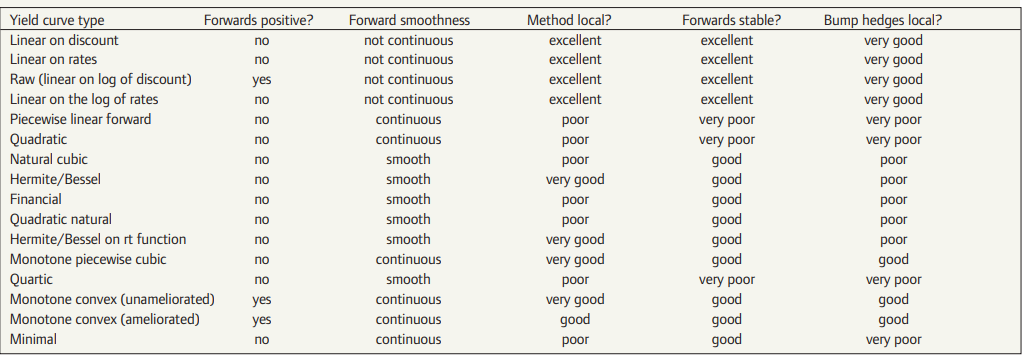
\includegraphics[width=1\textwidth]{Tables/InterpolationMethods.png}
        \caption{Interpolation Methods}
        \label{table:Interpolation_Methods}
    \end{table}
    
    \noindent
    Hagan and West \cite{hagan2008methods} highlight that the choice of interpolation scheme is critical not just for smoothness but also for preventing arbitrage opportunities. The structure of the forward rate curve  $f(t)$ is the primary visual and mathematical indicator of the quality of an interpolation method. This is because a negative forward rate implies that the discount factor function $Z(t)$ is not monotonically decreasing, which allows for arbitrage opportunities \cite{hagan2008methods}.

    \noindent
    Given this segmentation, the construction of the continuous discount curve $P(t,T)$ proceeds via a recursive algorithm that solves for discount factors sequentially, moving from the shortest maturities to the longest. Let $t$ denote the valuation (reference) date. The market provides a set of quoted instruments (deposits, FRAs, swaps) with strictly increasing terminal dates $\{d_i\}_{i=1}^n$, called \emph{calibration dates}. Each instrument contributes one pricing equation whose unknown is the discount factor $P(t,d_i)$. 
    
    \begin{itemize}
        \item Step 1: Initialization set $P(0,0) =1$
        \item Step 2: The curve is extended using deposits and FRAs. For the first instruments (typically up to 1 year), calculate $P(0,T_i)$ directly from the forward rate $F(0,T_{i-1},T_i)$
        \begin{equation} \label{eq:fraDF}
            P(0,T_i) = \frac{P(0,T_{i-1})}{1+F(0,T_{i-1},T_{i})\tau(T_{i-1},T_i)}
        \end{equation}
        \item Step 3: Assume the discount curve has been constructed up to time $T_{k-1}$.
        To solve for the discount factor at $T_k$ using a par swap with fixed rate $S_k$, we use the par swap equation. In a single-curve framework, the present value of the floating leg equals $1 - P(0,T_k)$ (under the standard no-notional-exchange logic). Equating floating and fixed legs gives
        \begin{equation}\label{eq:swap-core}
          1 - P(0,T_k)
          \;=\;
          S_k \sum_{i=1}^{k} \tau_i \, P(0,T_i),
        \end{equation}
        where $\alpha_i$ are the accrual fractions for the fixed-leg payments. Since $P(0,T_1),\dots,P(0,T_{k-1})$ are known from previous steps, we isolate $P(0,T_k)$ from \eqref{eq:swap-core}. If the swap includes intermediate payment dates $T_j$ with $T_{k-1} < T_j < T_k$ for which discount factors are not yet explicitly solved, we express these as functions of the known curve and the unknown target $P(0,T_k)$ via the chosen interpolation operator $\varphi$:
        \begin{equation}\label{eq:interp}
          P(0,T_j) \;=\; \varphi\!\big( T_j;\, \{(T_i,P(0,T_i))\}_{i=0}^{k-1},\, P(0,T_k) \big),
          \qquad T_{k-1} < T_j < T_k.
        \end{equation}
        Substituting \eqref{eq:interp} into \eqref{eq:swap-core} yields a (generally) nonlinear equation in the single unknown $P(0,T_k)$, which is then solved numerically. In the common case where all payment dates are on the existing grid (i.e., no intermediate unknowns), \eqref{eq:swap-core} reduces to a linear equation with the closed-form solution
        \begin{equation}\label{eq:swap-closed-form}
          P(0,T_k)
          \;=\;
          \frac{\,1 \;-\; S_k \displaystyle\sum_{i=1}^{k-1} \alpha_i P(0,T_i)\,}
               {\,1 + S_k \alpha_k\,}.
        \end{equation}
        \noindent 
        Repeat the recursive step for successive maturities until the longest instrument is exactly repriced, yielding a complete term structure $T \mapsto P(0,T)$. Between calibration dates, obtain a continuous curve using the selected interpolation method (e.g., linear in $\ln P(0,t)$, monotone convex).
    \end{itemize}

    \noindent
    The yield curve and the discount curve obtained from bootstrapping carry the same term-structure information but in different representations. The bootstrap algorithm produces discount factors $P(t,T)$, which are the fundamental inputs for pricing. The yield curve $R(t,T)$ is simply an alternative representation of the same term-structure information, obtained by converting discount factors into annualised zero rates under a chosen compounding convention.
    \begin{definition}[Yield Curve]\label{def:yield_curve}
    The \textbf{Yield Curve} at time \( t \) is the graph of the function:
    \begin{equation}
        T \mapsto R(t,T) \quad \text{for } T \geq t.
    \end{equation} 

    \end{definition}
    \noindent
    Practitioners pay attention to the shape of the yield curve: 
    \begin{itemize}
        \item \textbf{Upward-sloping (normal) yield curve:} Long-term yields exceed short-term yields, typically reflecting expectations of future economic growth, rising interest rates, and compensation for maturity and inflation risk.

        \item \textbf{Flat yield curve:} Short- and long-term yields are broadly similar, usually indicating a transition phase in the economy or uncertainty about future monetary policy, often preceding turning points in the interest rate cycle.
        
        \item \textbf{Inverted yield curve:} Short-term yields exceed long-term yields, commonly interpreted as a signal of expected economic slowdown or recession, as markets anticipate falling future interest rates.

        \item \textbf{Humped yield curve:} Medium-term yields exceed both short-term and long-term yields, producing a hump in the curve. This shape typically arises when markets anticipate near-term interest rate increases followed by a longer-term decline, or during periods of elevated uncertainty about the medium-term economic outlook. 
    \end{itemize}

    \begin{figure}[h!]
        \centering
        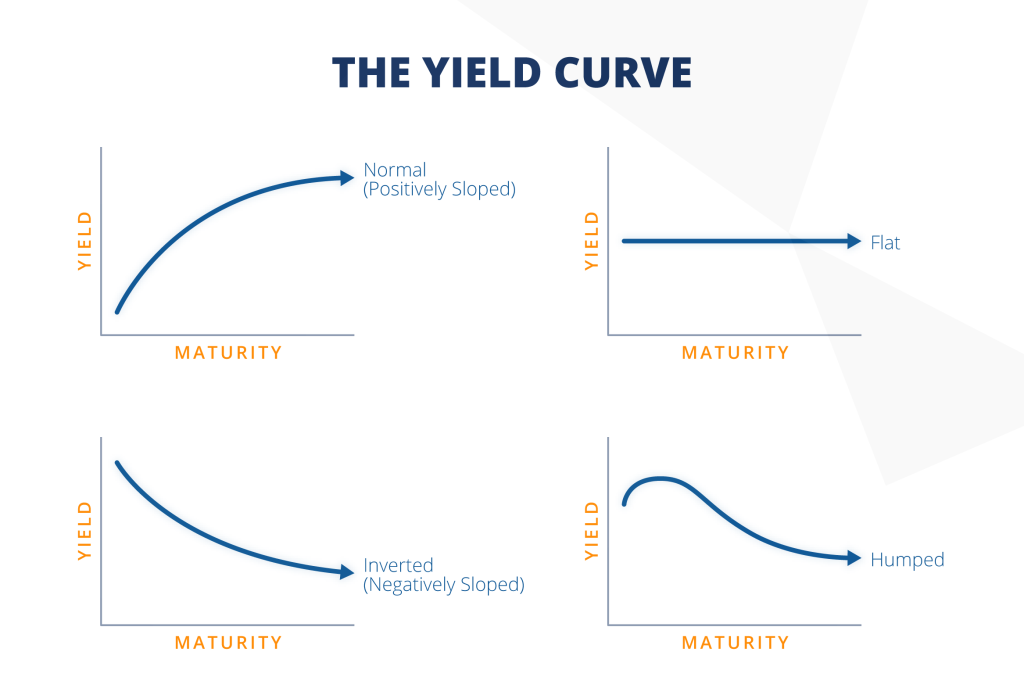
\includegraphics[width=0.9\textwidth]{Images/yield_curves_shapes.png}
        \caption{Typical yield curve shapes: upward-sloping (normal), flat, and inverted.}
        \label{fig:yield_curve_shapes}
    \end{figure}

    \subsection*{Parametric Curve Estimation: The Svensson Model}

    \noindent
    The bootstrapping algorithm above produces discount factors that exactly reprice all calibration instruments, but the resulting curve is piecewise in structure and sensitive to the choice of interpolation scheme. For applications requiring a globally smooth and differentiable term structure, an alternative approach is to fit a parametric functional form directly to observed market rates. Parametric models sacrifice exact repricing in favour of parsimony and smoothness, and are widely used by central banks for monetary policy analysis and for constructing initial term structures that serve as inputs to short-rate models \cite{bis2005zerocoupon}. The most widely adopted specification is the Svensson (1994) extension of the Nelson-Siegel model, which decomposes the instantaneous forward curve into four factor loadings and two decay parameters \cite{svensson1994estimating}.

    \noindent
    The Svensson model specifies the instantaneous forward rate $f(0,t)$ as:
    \begin{equation}\label{eq:svensson-forward}
        f(0,t) = \beta_0 + \beta_1 e^{-t/\tau_1}
                + \beta_2 \frac{t}{\tau_1} e^{-t/\tau_1}
                + \beta_3 \frac{t}{\tau_2} e^{-t/\tau_2}
    \end{equation}
    Integrating over $[0,t]$ and dividing by $t$ yields the corresponding continuously compounded zero rate:
    \begin{equation}\label{eq:svensson-zero}
        R(0,t) = \beta_0
                + \beta_1 \frac{1-e^{-t/\tau_1}}{t/\tau_1}
                + \beta_2 \left(\frac{1-e^{-t/\tau_1}}{t/\tau_1} - e^{-t/\tau_1}\right)
                + \beta_3 \left(\frac{1-e^{-t/\tau_2}}{t/\tau_2} - e^{-t/\tau_2}\right)
    \end{equation}
    The six parameters carry direct economic interpretations:
    \begin{itemize}
        \item $\beta_0 > 0$: the long-run level of interest rates, to which the curve converges as $t \to \infty$
        \item $\beta_1$: the slope factor, determining the spread between short- and long-term rates; a negative value produces an upward-sloping curve
        \item $\beta_2$: the first curvature factor, generating a hump or trough that peaks near maturity $\tau_1$
        \item $\beta_3$: the second curvature factor, allowing an additional hump near maturity $\tau_2$, extending the flexibility of the original Nelson-Siegel specification
        \item $\tau_1, \tau_2 > 0$: decay parameters controlling how quickly the slope and curvature contributions revert to zero with increasing maturity
    \end{itemize}
    The parameters are estimated by minimising the sum of squared deviations between model-implied and observed market zero rates across calibration maturities \cite{svensson1994estimating}:
    \begin{equation}\label{eq:svensson-calib}
        \min_{\beta_0,\,\beta_1,\,\beta_2,\,\beta_3,\,\tau_1,\,\tau_2}
        \sum_{i} \left(R^{\mathrm{market}}(0,t_i) - R(0,t_i)\right)^2
    \end{equation}

    \noindent
    The Svensson model is of particular relevance to the Hull-White framework developed in this study. Calibrating the time-dependent drift $\theta(t)$ to the initial term structure requires evaluating $\partial f(0,t)/\partial t$, since the exact expression for $\theta(t)$ depends on the slope of the initial forward curve at every point in time. A piecewise bootstrapped curve, being discontinuous between calibration pillars, yields an unreliable numerical derivative at those points. The Svensson forward rate in Equation~\eqref{eq:svensson-forward} is smooth and analytically differentiable everywhere, supplying a stable and consistent input to the Hull-White calibration described in the methodology chapter.

    \subsection*{HJM Framework}
    \noindent
    The evolution of term structure modelling represents a structural shift in how interest rate models are formulated. Early equilibrium models, such as Vasicek (1977) and Cox-Ingersoll-Ross (1985), specified the dynamics of the instantaneous short rate $r(t)$ under a risk-neutral measure and derived the yield curve as an output \cite{Green_2016}. This endogenous approach had a fundamental practical deficiency: because the initial yield curve was a model output rather than an input, these models could not exactly reprice the liquid benchmark instruments observed in the market, introducing systematic pricing errors that undermined their use in derivative valuation \cite{oosterlee2019mathematical}. The HJM framework addressed this by reversing the modelling direction entirely. \\

    \noindent
    Before stating the HJM dynamics, we formalise the object being modelled. The term structure of interest rates is not a single scalar but a continuum of rates indexed by maturity, admitting three equivalent representations.

    \begin{definition}[Term Structure]\label{def:term_structure}
    The \textbf{term structure of interest rates} at time $t$ is the collection of discount factors $\{P(t,T) : T \geq t\}$, or equivalently the family of mappings
    \begin{equation}
        T \mapsto R(t,T), \qquad T \mapsto f(t,T), \qquad T \mapsto P(t,T), \quad T \geq t,
    \end{equation}
    where $R(t,T)$ is the continuously compounded zero rate, $f(t,T)$ is the instantaneous forward rate, and $P(t,T)$ is the zero-coupon bond price. Each representation encodes the same term-structure information and must be consistent with observed market prices and the no-arbitrage conditions of Theorems~\ref{thm:FTAP} and~\ref{thm:SFTAP}.
    \end{definition}

    \noindent
    Given any one of the three representations, the other two are recovered without loss of information. The zero-coupon bond price $P(t,T)$ is the most fundamental, since it is the discounting kernel for future cash flows, but the instantaneous forward rate $f(t,T)$ is the most convenient state variable for modelling the dynamics of the entire curve, as it is directly observable in the limit of the simple compounded forward rate. \\

    \noindent
    The Heath-Jarrow-Morton (HJM) framework \cite{kwok2008mathematical} resolved the endogeneity problem by taking the initial forward rate curve $f(0,\cdot)$ as a given infinite-dimensional input, calibrated directly to market data, and specifying only the stochastic dynamics of its evolution through time. This ensures an automatic, exact fit to the observed term structure at $t = 0$. Within this framework, the Hull-White (1990) model emerges not merely as an extension of Vasicek but as a specific, Markovian restriction of the general HJM dynamics that retains analytic tractability while preventing arbitrage \cite{Green_2016}. \\

    \noindent
    Under the smoothness assumption on $P(t,T)$ in Definition~\ref{def:zcb}, the instantaneous forward rate is well-defined for all $T \geq t$ and is related to the simple compounded forward rate $F(t,T,T+\Delta T)$ introduced in Definition~\ref{def:forward_rate} by taking the limit as the accrual period shrinks to zero \cite{brigo2001interest}.

    \begin{definition}[Instantaneous Forward Rate] \label{def:inst_forward_rate}
    The \textbf{instantaneous forward rate} $f(t,T)$ prevailing at time $t$ for maturity $T > t$ is defined by
    \begin{equation}
        f(t,T) = \lim_{\Delta T \to 0} F(t,T,T+\Delta T) = -\frac{\partial}{\partial T} \ln P(t,T)
    \end{equation}
    \end{definition}

    \noindent
    The zero-coupon bond price is recovered from the instantaneous forward rate by integration:
    \begin{equation}
        P(t,T) = \exp\!\left(-\int_t^T f(t,u)\,du\right)
    \end{equation}
    The instantaneous short rate $r(t)$ is the limiting case at the current time:
    \begin{equation}
        r(t) = f(t,t) = \lim_{T \downarrow t} R(t,T)
    \end{equation}
    These relationships confirm that the instantaneous forward curve $T \mapsto f(t,T)$ is a complete description of the term structure: it determines all bond prices and all spot rates simultaneously. \\

    \noindent
    The HJM framework models the stochastic evolution of the entire forward curve simultaneously. Under the risk-neutral measure $\mathbb{Q}$, the dynamics of $f(t,T)$ for all maturities $T \geq t$ are governed by the SDE
    \begin{equation}
        df(t,T) = \alpha(t,T)\,dt + \sigma(t,T)\,dW(t)
    \end{equation}
    where $W(t)$ is a standard Brownian motion under $\mathbb{Q}$ and $\sigma(t,T)$ is the volatility structure. The central contribution of Heath, Jarrow, and Morton is that, under the risk-neutral measure, the drift $\alpha(t,T)$ is not a free modelling choice but is uniquely determined by the volatility structure through the no-arbitrage drift condition. For a one-factor model,
    \begin{equation}
        \alpha(t,T) = \sigma(t,T)\int_t^T \sigma(t,u)\,du
    \end{equation}
    This result means the modeller specifies only $\sigma(t,T)$ and the initial curve $f(0,T)$; the no-arbitrage requirement then determines the entire future evolution of the term structure \cite{kwok2008mathematical}. However, for a general choice of $\sigma(t,T)$, the HJM dynamics are non-Markovian: the state of the forward curve at time $t$ depends on the full path of $W$, not merely on its current value. In a lattice implementation, this produces non-recombining trees whose node count grows exponentially with the number of time steps, rendering the general framework computationally intractable for large derivative portfolios \cite{Green_2016, Hull_2018}.

    \noindent
    The Hull-White model resolves this by imposing an economically motivated constraint on the volatility structure \cite{Hull_2018}. If $\sigma(t,T)$ is chosen to be exponentially decaying in the time-to-maturity $(T-t)$,
    \begin{equation}
        \sigma(t,T) = \sigma\,e^{-a(T-t)}
    \end{equation}
    then the HJM dynamics collapse to a Markovian system driven by the single state variable $r(t)$ \cite{kwok2008mathematical}. This volatility structure has a direct economic interpretation: shocks to the short end of the forward curve dampen at rate $a$ as maturity increases, encoding mean reversion directly into the curve dynamics \cite{gupta2005pricing}. Under this specification, the short rate follows the SDE
    \begin{equation}
        dr(t) = [\theta(t) - a\,r(t)]\,dt + \sigma\,dW(t)
    \end{equation}
    where $a > 0$ is the mean reversion speed, $\sigma > 0$ is the instantaneous volatility, and $\theta(t)$ is a deterministic function calibrated to fit the initial term structure exactly. This calibration requires the initial instantaneous forward curve and its time derivative, which the Svensson parametrisation introduced above supplies analytically \cite{brigo2001interest}:
    \begin{equation}\label{eq:theta}
        \theta(t) = \frac{\partial f^M(0,t)}{\partial t} + a\,f^M(0,t)
                  + \frac{\sigma^2}{2a}\!\left(1 - e^{-2at}\right)
    \end{equation}
    where $f^M(0,t)$ denotes the market-implied initial instantaneous forward rate. This formulation reduces the entire state of the term structure to the single variable $r(t)$, permitting efficient simulation via recombining trinomial trees and Monte Carlo methods. \\

    \noindent
    Since the Hull-White SDE is linear in $r(t)$, it admits an exact closed-form solution requiring no approximation, a property that sets it apart from nonlinear short-rate models such as Cox-Ingersoll-Ross, where explicit solutions do not exist in general \cite{brigo2001interest}. The standard technique is to multiply both sides of the SDE by the integrating factor $e^{at}$, which converts the left-hand side into a perfect differential via It\^{o}'s product rule:
    \begin{equation}
        d\!\left(e^{at}r(t)\right) = e^{at}\theta(t)\,dt + \sigma e^{at}\,dW(t)
    \end{equation}
    Integrating both sides from $s$ to $t$ and dividing through by $e^{at}$ yields the explicit solution:
    \begin{equation}\label{eq:hw-solution}
        r(t) = e^{-a(t-s)}r(s) + \int_s^t e^{-a(t-u)}\theta(u)\,du
               + \sigma\int_s^t e^{-a(t-u)}\,dW(u)
    \end{equation}

    \noindent
    The solution decomposes the short rate into three additive components, each with a clear economic interpretation. The first term, $e^{-a(t-s)}r(s)$, is the mean-reverting decay of the current short rate: the factor $e^{-a(t-s)}$ pulls the current value exponentially towards zero at rate $a$, so that the influence of today's rate diminishes as the horizon lengthens. The second term is the accumulated contribution of the deterministic drift $\theta(u)$, weighted by the same exponential decay, representing the path along which the expected short rate is continuously attracted towards the market-implied forward curve. The third term is the stochastic component: a weighted sum of Brownian increments $dW(u)$ accumulated from $s$ to $t$, with older shocks discounted more heavily than recent ones. In plain terms, the short rate at any future time is the net result of where it starts, where the market implies it is heading, and the random disturbances that arrive along the way \cite{Hull_2018}. \\

    \noindent
    Because the stochastic integral in Equation~\eqref{eq:hw-solution} is a linear functional of Brownian motion, it is Gaussian by construction. This means that, conditional on the filtration $\mathcal{F}_s$, the short rate $r(t)$ is normally distributed \cite{brigo2001interest}:
    \begin{equation}\label{eq:hw-dist}
        r(t)\,|\,\mathcal{F}_s \;\sim\; \mathcal{N}\!\left(\mu(s,t),\; V(s,t)\right)
    \end{equation}
    with conditional mean and variance:
    \begin{equation}\label{eq:hw-mean}
        \mu(s,t) = e^{-a(t-s)}r(s) + \int_s^t e^{-a(t-u)}\theta(u)\,du
    \end{equation}
    \begin{equation}\label{eq:hw-var}
        V(s,t) = \frac{\sigma^2}{2a}\!\left(1 - e^{-2a(t-s)}\right)
    \end{equation}
    The mean $\mu(s,t)$ reflects the two deterministic forces already identified in the explicit solution: the decayed current rate and the forward-curve-implied drift. The variance $V(s,t)$ increases monotonically from zero at $t = s$ and saturates at $\sigma^2/(2a)$ as $t \to \infty$. This saturation is a direct consequence of mean reversion: unlike a driftless Brownian motion, where uncertainty accumulates without bound, mean reversion prevents the short rate from wandering arbitrarily far from the forward curve, bounding the long-run uncertainty by the ratio of volatility to mean reversion speed \cite{kwok2008mathematical}. \\

    \noindent
    The Gaussian structure of the solution has three direct consequences for this study. First, since bond prices take the form $P(t,T) = A(t,T)\,e^{-B(t,T)r(t)}$ and $r(t)$ is normally distributed, bond prices are lognormally distributed. This is precisely the property that enables the closed-form ATSM expressions derived below and underpins the analytical swaption and cap pricing formulae used for calibrating $a$ and $\sigma$ to market data \cite{brigo2001interest}. \\

    \noindent
    Second, the normal distribution assigns positive probability to negative values of $r(t)$ for all $t > s$. Negative short rates are inconsistent with the classical interpretation of the money market account as a locally riskless investment accumulating at the prevailing short rate, and represent a theoretical limitation of the Gaussian specification \cite{Green_2016}. In practice, the probability of negative rates under calibrated Hull-White parameters is small for typical upward-sloping or flat term structures, and the analytical tractability of the Gaussian model is considered to outweigh this limitation for the IRS portfolio considered in this study. \\

    \noindent
    Third, and most directly relevant to the numerical methodology, the exact conditional distribution in Equation~\eqref{eq:hw-dist} means that Monte Carlo simulation of the short rate requires no time-stepping approximation. At each simulation step $[t_i, t_{i+1}]$ with $\Delta t = t_{i+1} - t_i$, the short rate is drawn exactly from its conditional distribution \cite{brigo2001interest}:
    \begin{equation}\label{eq:hw-mc}
        r(t_{i+1}) = e^{-a\Delta t}r(t_i) + \mu_{\Delta}(t_i)
                   + \sqrt{V(t_i,\,t_{i+1})}\;Z_i,
                   \quad Z_i \overset{\text{iid}}{\sim} \mathcal{N}(0,1)
    \end{equation}
    where $\mu_{\Delta}(t_i) = \int_{t_i}^{t_{i+1}} e^{-a(t_{i+1}-u)}\theta(u)\,du$ is the deterministic drift contribution over the step. Unlike the Euler-Maruyama scheme, which introduces a strong-order bias proportional to $\Delta t$, this discretisation is exact: the only source of error in the simulated short rate paths is Monte Carlo sampling variance, which diminishes at the standard $1/\sqrt{N}$ rate as the number of simulated paths $N$ increases \cite{kwok2008mathematical}. This exact simulation scheme is used directly in the exposure and xVA calculations of the methodology chapter. \\

    \noindent
    A further analytical advantage of the Hull-White model is its classification as an Affine Term Structure Model (ATSM), which yields closed-form zero-coupon bond prices. Given $r(t)$, the time-$t$ price of a zero-coupon bond maturing at $T$ takes the exponential affine form
    \begin{equation}
        P(t,T) = A(t,T)\,\mathrm{e}^{-B(t,T)\,r(t)}
    \end{equation}
    where the deterministic functions $B(t,T)$ and $A(t,T)$ are given by \cite{brigo2001interest}
    \begin{equation}\label{eq:hw-B}
        B(t,T) = \frac{1 - e^{-a(T-t)}}{a}
    \end{equation}
    \begin{equation}\label{eq:hw-lnA}
        \ln A(t,T) = \ln\frac{P^M(0,T)}{P^M(0,t)} - B(t,T)\,f^M(0,t)
                   - \frac{\sigma^2}{4a}\!\left(1 - e^{-2at}\right)B(t,T)^2
    \end{equation}
    The affine structure admits closed-form expressions for European swaptions and caps, making model calibration tractable: the parameters $a$ and $\sigma$ are typically estimated by fitting to the ``diagonal'' of the swaption volatility matrix or a strip of at-the-money cap volatilities \cite{brigo2001interest}. The principal limitation of the one-factor specification is that all instantaneous forward rates are driven by a single Brownian motion, implying perfect instantaneous correlation across the curve. This precludes exact replication of portfolios sensitive to non-parallel yield curve movements such as twists and butterflies, a limitation acknowledged in the calibration discussion of the following chapter.

    \chapter{Counterparty Credit Risk and xVAs}

    \noindent
    The post-crisis derivatives market fundamentally altered the way in which banks price and manage OTC derivatives. Prior to 2008, the prevailing assumption in quantitative finance was that counterparties to a derivative transaction were effectively default-free, allowing the standard risk-neutral price to serve as a complete valuation \cite{Green_2016}. The collapse of Lehman Brothers in September 2008 made explicit what had previously been treated as negligible: every OTC derivative trade carries bilateral exposure to counterparty default, and that exposure carries an economic cost that must be reflected in the price \cite{Gregory_2015}. This chapter formalises the mathematical framework underlying that cost. Section~\ref{sec:ccr} defines the exposure measures central to counterparty risk quantification. Section~\ref{sec:credit-mitigants} introduces the legal and contractual mechanisms that reduce but do not eliminate counterparty exposure. Section~\ref{sec:cva-dva} derives the Credit Valuation Adjustment (CVA) and Debit Valuation Adjustment (DVA) as expectation integrals over simulated exposure profiles. These integrals are evaluated numerically in Chapter~7 using the Hull-White Monte Carlo engine introduced in Chapter~5.

    \section*{Counterparty Credit Risk}
    \label{sec:ccr}

    \noindent
    Counterparty credit risk (CCR) is the risk that a counterparty to a financial transaction will fail to fulfil its payment obligations before the final settlement of the trade \cite{Green_2016}. Unlike loan credit risk, where exposure is one-directional and fixed at inception, the exposure arising from a derivatives transaction is bilateral and dynamic: the direction of net exposure reverses as market rates evolve, and its magnitude can grow substantially over the life of a long-dated contract \cite{cesari2009modelling, Gregory_2015}. \\

    \noindent
    The central quantity in CCR measurement is the \textbf{exposure at default} (EAD), defined as the net amount owed by the defaulting counterparty at the instant of default. Since OTC derivatives can carry both positive and negative mark-to-market value, the EAD from the perspective of party $A$ is
    \begin{equation}
        \text{EAD}(t) = \max\!\left(V(t),\, 0\right),
        \label{eq:EAD}
    \end{equation}
    where $V(t)$ denotes the mark-to-market value of the netted derivative portfolio at time $t$ \cite{Gregory_2015}. When $V(t) < 0$, party $A$ owes the counterparty money and no credit exposure exists from $A$'s perspective at that instant. \\

    \noindent
    Since default can occur at any point during the tenor of the contract, CCR management requires a forward-looking view of the exposure profile. Two expectation-based measures are standard \cite{canabarro2003measuring, zhu2007guide}. The \textbf{expected positive exposure} (EPE) and \textbf{expected negative exposure} (ENE) at time $t$ are defined, respectively, as
    \begin{align}
        \text{EPE}(t) &= \mathbb{E}_t\!\left[\max\!\left(V(t),\, 0\right)\,\middle|\,\mathcal{F}_t\right], \label{eq:EPE} \\[4pt]
        \text{ENE}(t) &= \mathbb{E}_t\!\left[\max\!\left(-V(t),\, 0\right)\,\middle|\,\mathcal{F}_t\right]. \label{eq:ENE}
    \end{align}
    Both quantities are non-negative by construction. The EPE profile captures the average exposure of party $A$ to counterparty default, whilst the ENE profile captures the average exposure of the counterparty to party $A$'s own default. The EPE feeds directly into the CVA calculation and the ENE into the DVA calculation, as formalised in Section~\ref{sec:cva-dva}. \\

    \noindent
    In the event of default, the non-defaulting party does not lose the full EAD. A fraction of the outstanding claim, the \textbf{recovery rate} $R \in [0,1]$, is recovered through the bankruptcy process. The complementary quantity
    \begin{equation}
        \text{LGD} = 1 - R
        \label{eq:LGD}
    \end{equation}
    is the \textbf{loss given default}, the true economic loss per unit of exposure \cite{Green_2016}. In the bilateral setting of this study, separate recovery rates $R_C$ and $R_B$ are assigned to the counterparty and to the bank respectively, with corresponding losses given default $\text{LGD}_C = 1 - R_C$ and $\text{LGD}_B = 1 - R_B$. \\

    \noindent
    A further complication in CCR arises when the exposure is correlated with the creditworthiness of the defaulting party. \textbf{Wrong-way risk} occurs when the exposure to a counterparty increases precisely as the counterparty's credit quality deteriorates, amplifying the potential loss beyond what is implied by an unconditional EPE profile \cite{Green_2016}. For interest rate swaps, a corporate counterparty that pays fixed and receives floating may face financial stress in high-rate environments, exactly when the swap carries positive value to the bank. \textbf{Right-way risk} is the converse: a favourable correlation between exposure and credit quality reduces realised losses relative to the unconditional EPE \cite{Gregory_2015}. This study assumes independence between the short-rate process and the default intensities $\lambda_C$ and $\lambda_B$, setting aside wrong-way and right-way risk effects in order to isolate the contribution of the Hull-White interest rate model to the exposure profile.

    \section*{Credit Risk Mitigants}
    \label{sec:credit-mitigants}

    \noindent
    Several contractual arrangements exist to reduce counterparty credit exposure in the OTC derivatives market. \\

    \noindent
    \textbf{Close-out netting.} A close-out netting agreement, enshrined in the ISDA Master Agreement, provides the legal basis for offsetting positive and negative mark-to-market values across a portfolio of trades between two counterparties at the moment one party defaults \cite{Green_2016}. Without netting, the surviving party must honour trades with negative value whilst filing as an unsecured creditor for trades with positive value; under netting, only the net portfolio value constitutes the EAD. Research by ISDA suggests that netting can reduce aggregate credit exposure by as much as 85\% for diversified derivatives portfolios \cite{brigo2013counterparty}. \\

    \noindent
    \textbf{Collateral and the CSA.} A Credit Support Annex (CSA), attached to the ISDA Master Agreement, governs the periodic posting of collateral between counterparties in support of the mark-to-market of the portfolio. The call frequency, minimum transfer amount, eligible collateral types, and counterparty-specific thresholds are all specified contractually \cite{Green_2016}. A CSA does not eliminate credit exposure entirely: the residual exposure over the margin period of risk, the interval between the last collateral posting and the close-out of the position, generates a smaller but non-zero CVA even for collateralised trades. \\

    \noindent
    For the purposes of this study, we adopt the clean exposure assumption: no CSA is in place, and the full expected positive exposure profile is exposed to counterparty default. This is consistent with the bilateral, uncollateralised interest rate swap transactions that motivate the xVA calculations in Chapter~7, and it ensures that the computed CVA and DVA reflect the unmitigated bilateral credit adjustment.

    \section*{Credit and Debit Valuation Adjustments}
    \label{sec:cva-dva}

    \noindent
    The credit-risky value of a bilateral derivative differs from its default-free, risk-neutral counterpart whenever either counterparty faces a non-zero probability of default. Burgard and Kjaer \cite{pde_2011, burgard2011balance} derived the governing PDE for this bilateral credit-risky value via a replication argument under the risk-neutral measure, accounting separately for the cost of the counterparty's default through CVA and the benefit of the bank's own default through DVA.

    \begin{thmbox}{}{thm:credit-risky-pde}
        The price of a credit risky derivative trade satisfies the following PDE
        \[
        \left\{
        \begin{array}{l}
            \dfrac{\partial \hat{V}}{\partial t} + \mathcal{A}_t \hat{V} - r\hat{V} = \lambda_C(1-R_C)V^+ + \lambda_B(1-R_B)V^- \\[10pt]
            \hat{V}_T = V_T \text{ is the final payoff of the derivative}
        \end{array}
        \right.
        \]
        where the risk-free price satisfies the Black-Scholes PDE
        \[
        \left\{
        \begin{array}{l}
            \dfrac{\partial V}{\partial t} + \mathcal{A}_t V - rV = 0 \\[10pt]
            V_T \text{ is the final payoff of the derivative}
        \end{array}
        \right.
        \]
        and the parabolic differential operator is given by
        \[
            \mathcal{A}_t = \frac{1}{2}\sigma^2 S^2 \frac{\partial^2}{\partial S^2} + rS\frac{\partial}{\partial S}.
        \]
    \end{thmbox}

    \noindent
    In the bilateral PDE, $\hat{V}$ denotes the credit-risky derivative price, $V$ is the default-free risk-neutral price, $\lambda_C$ and $\lambda_B$ are the risk-neutral default intensities (hazard rates) of the counterparty and the bank, $R_C$ and $R_B$ are their respective recovery rates, and $V^+ = \max(V,0)$ and $V^- = \min(V,0)$ denote the positive and negative parts of the default-free price. The operator $\mathcal{A}_t$ is the infinitesimal generator of the underlying state process; for the Hull-White interest rate model considered in this study it takes the form $\mathcal{A}_t = [\theta(t) - ar]\,\partial_r + \tfrac{1}{2}\sigma^2\,\partial_{rr}$, whilst for an equity underlying it reduces to the Black-Scholes generator as written above. The structure of the bilateral PDE is unchanged across both settings. The right-hand side decomposes into two channels: the term $\lambda_C(1-R_C)V^+$ is the CVA source, which reduces the credit-risky price relative to the default-free price when the portfolio has positive value to the bank; and the term $\lambda_B(1-R_B)V^-$ is the DVA source, which increases the credit-risky price when the portfolio has negative value to the bank, since the bank's own default then constitutes a benefit to the surviving counterparty. \\

    \noindent
    Applying the Feynman-Kac theorem to the bilateral PDE and taking expectations under the risk-neutral measure $\mathbb{Q}$, the bilateral credit-risky price decomposes as \cite{pde_2011, brigo2013counterparty}
    \begin{equation}
        \hat{V}(t) = V(t) - \text{CVA}(t) + \text{DVA}(t).
        \label{eq:bilateral-price}
    \end{equation}
    The \textbf{Credit Valuation Adjustment} is the expected loss to the bank from the counterparty's default, weighted by the counterparty's default intensity:
    \begin{equation}
        \text{CVA}(t) = \text{LGD}_C \int_t^T \text{EPE}(s)\,\lambda_C(s)\,ds.
        \label{eq:CVA}
    \end{equation}
    The \textbf{Debit Valuation Adjustment} is the expected gain to the bank from its own default, weighted by the bank's default intensity:
    \begin{equation}
        \text{DVA}(t) = \text{LGD}_B \int_t^T \text{ENE}(s)\,\lambda_B(s)\,ds.
        \label{eq:DVA}
    \end{equation}
    CVA is always non-negative and reduces the bilateral price; DVA is always non-negative and increases it. The combined \textbf{bilateral credit valuation adjustment} (BCVA) is
    \begin{equation}
        \text{BCVA}(t) = \text{CVA}(t) - \text{DVA}(t),
        \label{eq:BCVA}
    \end{equation}
    so that $\hat{V}(t) = V(t) - \text{BCVA}(t)$. When $\text{BCVA} > 0$ the net credit adjustment reduces the trade value; when $\text{BCVA} < 0$ the DVA benefit dominates. The sign of BCVA depends on the relative default intensities and recovery rates of both parties and on the direction of the net exposure profile \cite{Green_2016, Gregory_2015}. \\

    \noindent
    The EPE and ENE integrals in equations~\eqref{eq:CVA} and~\eqref{eq:DVA} are not available in closed form for a general stochastic term structure. They are evaluated numerically in Chapter~7 by simulating the Hull-White short rate along Monte Carlo paths and computing the expected exposures at each simulation date using the closed-form IRS valuation established in Chapter~5.

    \chapter{Neural Networks and Deep Learning}

    The tractability of derivative pricing under classical models rests on analytical or semi-analytical solutions that are available only under restrictive assumptions. Under the xVA framework developed in the preceding chapter, pricing must be performed across thousands of Monte Carlo simulation paths for the purpose of computing exposure profiles, and the computational cost of re-pricing a full derivatives portfolio at each time step is severe. Neural networks offer a principled response to this challenge, a trained network can emulate the pricing function to high accuracy whilst evaluating at a fraction of the computational cost of the underlying model. This chapter develops the mathematical foundations of neural networks and deep learning that underpin the surrogate modelling methodology employed in this study.

    \section*{The Artificial Neuron}

    The artificial neuron is the atomic computational unit of a neural network. Inspired by the threshold-activation behaviour of biological neurons, the artificial neuron receives a vector of inputs $\mathbf{x} = (x_1, \ldots, x_m)^{\top}$, computes a weighted sum, and produces an output determined by whether that sum exceeds a threshold. Given weights $w_1, \ldots, w_m$ and threshold $\theta$, the neuron activates if

    \[
    h = \sum_{i=1}^{m} w_i x_i > \theta.
    \]

    \noindent 
    Reparameterising by absorbing the threshold as a bias $b = -\theta$, the activation condition becomes $\sum_{i=1}^{m} w_i x_i + b > 0$. The boundary $\sum_{i=1}^{m} w_i x_i + b = 0$ defines a hyperplane in $\mathbb{R}^m$, and the
    neuron partitions its input space into two half-spaces. This constitutes the linear discriminant, and it represents the simplest possible classifier \citep{goodfellow2016deep}. \\

    \noindent
    The perceptron learning rule adjusts weights in response to classification errors. Given input $\mathbf{x}$, target $t \in \{0, 1\}$, and current output $y \in \{0, 1\}$, the update is

    \[
    w_i \leftarrow w_i + \eta(t - y)\, x_i, \qquad b \leftarrow b + \eta(t - y),
    \]

    \noindent 
    where $\eta \in (0, 1)$ is the learning rate, a scalar controlling the magnitude of each correction. When the prediction is correct ($t = y$), no update occurs. When the neuron fires incorrectly, the weight vector is adjusted in the direction of $\mathbf{x}$ (or its negative), geometrically moving the separating hyperplane toward the misclassified point. The algorithm converges in finite time when the dataset is linearly separable \citep{goodfellow2016deep}. When it is not, a single neuron is insufficient: the mapping from inputs to outputs cannot be represented as a single linear discriminant, and a richer architecture is required. \\

    \section*{Multi-Layer Perceptrons}

    The limitation of the single-layer perceptron motivates the multi-layer perceptron (MLP). The XOR function illustrates the issue directly: no single hyperplane separates its positive inputs $(0,1)$ and $(1,0)$ from its negative inputs $(0,0)$ and $(1,1)$, yet two hyperplanes suffice. The MLP achieves this by introducing hidden layers: each hidden layer learns an intermediate representation, and the output layer combines those representations to produce the network's decision or prediction \citep{rumelhart1986learning}. \\


    \noindent
    An MLP with $L$ layers is specified as follows. The input layer carries the raw features $\mathbf{x} \in \mathbb{R}^{d_0}$. Each subsequent layer $k = 1, \ldots, L$ receives the activation vector $\mathbf{a}_{k-1}$ from the preceding layer, applies a weight matrix $W_k \in \mathbb{R}^{d_{k-1} \times d_k}$ and a bias vector $\mathbf{b}_k \in \mathbb{R}^{d_k}$, and passes the result through an activation function $g_k$:

    \[
    \mathbf{a}_k = g_k\!\left(\mathbf{a}_{k-1} W_k + \mathbf{b}_k\right).
    \]

    \noindent
    The output layer produces $\mathbf{y} = \mathbf{a}_L$. The collection of all weights and biases across layers is denoted $\mathbf{W}$, and training amounts to finding the values of $\mathbf{W}$ that minimise a chosen measure of prediction error on the training data.

    \begin{figure}[htbp]
    \centering
    \begin{tikzpicture}[
        neuron/.style={circle, draw=blue!60!black, fill=blue!8,
                       minimum size=0.72cm, inner sep=0pt, line width=0.6pt},
        conn/.style={-Stealth, gray!50, line width=0.35pt},
        lbl/.style={font=\small},
        dim/.style={font=\footnotesize\itshape, text=blue!60!black},
        >=Stealth
    ]
    % Input layer
    \foreach \i/\y in {1/1.2, 2/0.0, 3/-1.2}
        \node[neuron] (I\i) at (0, \y) {};
    % Hidden layer 1
    \foreach \i/\y in {1/1.8, 2/0.6, 3/-0.6, 4/-1.8}
        \node[neuron] (H1\i) at (3.0, \y) {};
    % Hidden layer 2
    \foreach \i/\y in {1/1.8, 2/0.6, 3/-0.6, 4/-1.8}
        \node[neuron] (H2\i) at (6.0, \y) {};
    % Output layer
    \node[neuron] (O) at (9.0, 0.0) {};
    % Connections
    \foreach \i in {1,2,3}
        \foreach \j in {1,2,3,4}
            \draw[conn] (I\i) -- (H1\j);
    \foreach \i in {1,2,3,4}
        \foreach \j in {1,2,3,4}
            \draw[conn] (H1\i) -- (H2\j);
    \foreach \i in {1,2,3,4}
        \draw[conn] (H2\i) -- (O);
    % Layer labels
    \node[lbl, above=0.55cm] at (0.0, 1.2) {Input};
    \node[lbl, above=0.55cm] at (3.0, 1.8) {Hidden};
    \node[lbl, above=0.55cm] at (6.0, 1.8) {Hidden};
    \node[lbl, above=0.55cm] at (9.0, 0.7) {Output};
    % Dimension labels
    \node[dim, below=0.5cm] at (0.0, -1.2) {$d_0$};
    \node[dim, below=0.5cm] at (3.0, -1.8) {$d_1$};
    \node[dim, below=0.5cm] at (6.0, -1.8) {$d_2$};
    \node[dim, below=0.5cm] at (9.0, -0.7) {$d_L$};
    % Weight matrix labels
    \node[font=\footnotesize, text=gray!65] at (1.5, 2.2) {$W_1$};
    \node[font=\footnotesize, text=gray!65] at (4.5, 2.2) {$W_2$};
    \node[font=\footnotesize, text=gray!65] at (7.5, 1.4) {$W_L$};
    \end{tikzpicture}
    \caption{A feedforward MLP with $L = 3$ layers. Each node applies an activation
    function to a weighted sum of the preceding layer's outputs. Weight matrices
    $W_k \in \mathbb{R}^{d_{k-1} \times d_k}$ connect adjacent layers; the layer
    widths $d_0, \ldots, d_L$ are illustrative.}
    \label{fig:mlp_architecture}
    \end{figure}

    \section*{Activation Functions}

    The activation function $g_k$ introduces the non-linearity that gives multi-layer networks their expressive power. Without it, a composition of affine transformations collapses to a single affine transformation regardless of depth, and the MLP reduces to a linear model. The choice of activation function affects both the expressiveness of the network and the stability of training. \\

    \begin{itemize}
    \item \textbf{Sigmoid.} The logistic sigmoid $\sigma(z) = (1 + e^{-z})^{-1}$ maps $\mathbb{R}$ into $(0, 1)$ and is differentiable everywhere. Its derivative satisfies $\sigma'(z) = \sigma(z)(1 - \sigma(z))$, a self-referential identity that simplifies gradient computation considerably. The sigmoid saturates for large $|z|$, causing gradients to vanish in deep networks and impeding learning.

    \item \textbf{Hyperbolic tangent.} The function $\tanh(z) = (e^z - e^{-z})/(e^z + e^{-z})$ maps $\mathbb{R}$ into $(-1, 1)$ and is zero-centred, which tends to produce better-conditioned gradient flow than the sigmoid. Its derivative is $\tanh'(z) = 1 - \tanh^2(z)$. Like the sigmoid, tanh saturates at large magnitudes.

    \item \textbf{Rectified linear unit (ReLU).} The activation $\mathrm{relu}(z) = \max(0, z)$ is piecewise linear with derivative 1 for $z > 0$ and 0 for $z < 0$ \citep{glorot2011deep}. It does not saturate on the positive half-line, which mitigates the vanishing gradient problem and enables effective training of deep architectures. The sub-gradient at $z = 0$ is set to 0 by convention. ReLU is the standard choice for hidden layers in modern deep learning.

    \item \textbf{Linear.} The identity $\mathrm{lin}(z) = z$ is appropriate at the output layer of a regression network, where the target is a real-valued quantity such as a derivative price and no bounding of the output is required. Using a linear output activation ensures the network can produce outputs of arbitrary magnitude and sign.
    \end{itemize}

    \noindent
    The choice of output activation is determined by the task structure. For derivative pricing, where the target is a real-valued price, a linear output activation is standard \citep{ruf2020neural}. For binary classification, a sigmoid output is appropriate, for multi-class outputs, the softmax function $\mathrm{softmax}(z_{n_i}) = e^{z_{n_i}} / \sum_{j} e^{z_{n_j}}$ maps the pre-activations to a valid probability distribution over classes.

    \section*{The Universal Approximation Theorem}

    The theoretical justification for using neural networks as surrogate pricing functions is provided by the Universal Approximation Theorem. The result was established independently by \citet{cybenko1989approximation} for sigmoid activations and generalised to a broad class of activation functions by \citet{hornik1989multilayer, hornik1991approximation}.

    \begin{theorem}[Universal Approximation]
    \label{thm:uat}
    Let $g: \mathbb{R} \to \mathbb{R}$ be a continuous, bounded, and non-constant function. For any continuous function $f: K \to \mathbb{R}$ defined on a compact set $K \subset \mathbb{R}^d$ and any $\varepsilon > 0$, there exists a
    single-hidden-layer neural network $F_\varepsilon$ with activation $g$ such that
    \[
    \sup_{\mathbf{x} \in K} |F_\varepsilon(\mathbf{x}) - f(\mathbf{x})| < \varepsilon.
    \]
    \end{theorem}

    \noindent
    The theorem guarantees that a sufficiently wide single-hidden-layer network can approximate any continuous function to arbitrary precision on a compact domain. It is the composition of non-linear activations, rather than any specific sigmoid form, that confers this universal approximating capacity \citep{hornik1991approximation}. \\

    \noindent
    Three qualifications are essential. First, the theorem establishes existence but not constructibility: it provides no guidance on the network width required or on whether a particular training procedure will locate the approximating parameter configuration. Second, the result applies to compact domains; pricing functions defined over unbounded parameter ranges require additional regularity arguments. Third, approximation in theory does not imply generalisation in practice. A network may fit training inputs arbitrarily well whilst performing poorly on out-of-sample scenarios. The practical question of generalisation is addressed by training methodology and regularisation, treated in subsequent sections. \\

    \noindent
    In the context of this study, Theorem~\ref{thm:uat} justifies using a neural network to emulate the Hull-White pricing function $V(r, t; \boldsymbol{\theta})$, where $\boldsymbol{\theta}$ denotes the vector of model and trade parameters. Under standard regularity conditions, this function is continuous in its arguments, and the domain of interest can be taken as a compact hypercube in the space of short-rate scenarios \citep{mrad2025differential}.

    \section*{The Feedforward Pass}

    The feedforward pass computes the network output for a given input. For node $n$, the pre-activation is

    \[
    z_n = \sum_{m} w_{mn} y_m + b_n,
    \]

    \noindent
    where the sum ranges over all nodes $m$ in the preceding layer and $y_m$ is the post-activation output of node $m$. The post-activation of node $n$ is $y_n = g_n(z_n)$. Collecting across layers, the computation reduces to the
    sequential matrix propagation $\mathbf{a}_k = g_k(\mathbf{a}_{k-1} W_k + \mathbf{b}_k)$ evaluated from $k = 1$ to $k = L$. \\

    \noindent
    During the forward pass, the activation values $a_n = y_n|_{\mathbf{x}, \mathbf{W}}$ are stored for subsequent use in backpropagation. Storing these intermediate values is the mechanism by which the chain rule is applied efficiently without recomputation. \\

    \section*{Loss Functions}

    Training requires a scalar measure of the discrepancy between the network output $\mathbf{y}$ and the training target $\mathbf{t}$. This is the loss function $L(\mathbf{y}, \mathbf{t})$. \\

    \noindent 
    For regression tasks, the standard choice is the \textbf{mean squared error} (MSE), derived from the sum-of-squares loss:

    \[
    L(\mathbf{y}, \mathbf{t}) = \frac{1}{2} \sum_{j} (y_j - t_j)^2,
    \]

    \noindent 
    where the sum ranges over all output nodes $j$ \citep{goodfellow2016deep}. MSE penalises large deviations quadratically and is appropriate when the target is a continuous quantity and errors of larger magnitude are disproportionately costly. In the surrogate pricing context, the target is the derivative price and the loss is MSE over the training portfolio. \\

    \noindent 
    For multi-class classification tasks with a softmax output, the cross-entropy loss is preferred:

    \[
    L_{CE}(\mathbf{y}, \mathbf{t}) = -\sum_{i=1}^{k} t_i \ln(y_i),
    \]

    \noindent 
    where $\mathbf{t}$ is one-hot encoded and the softmax outputs form a probability distribution over classes \citep{goodfellow2016deep}. The softmax/cross-entropy pairing admits a particularly clean gradient: the output-layer delta simplifies to $\delta_n = a_n - t_n$, with no activation-derivative factor. This arises from the cancellation between the softmax Jacobian and the logarithmic derivative of the cross-entropy, and it makes the gradient at the output proportional to the raw prediction error. \\

    \section*{Backpropagation}

    Gradient descent minimises the loss by iteratively adjusting each parameter in the direction of steepest descent. The update rule for edge weight $w_{mn}$ is

    \[
    w_{mn} \leftarrow w_{mn} - \eta \frac{\partial L}{\partial w_{mn}}\bigg|_{\mathbf{x}, \mathbf{t}, \mathbf{W}}.
    \]

    \noindent 
    Computing these partial derivatives efficiently across all parameters of a multi-layer network is the purpose of the backpropagation algorithm \citep{rumelhart1986learning}. Backpropagation is a direct application of the
    multivariable chain rule: gradient information is propagated backward through the network from the output layer to the input layer, accumulating the partial derivatives of each node's contribution to the loss. \\

    \noindent 
    The central quantity is the \textbf{delta value} at node $n$:

    \[
    \delta_n = \frac{\partial L}{\partial z_n}\bigg|_{\mathbf{x}, \mathbf{t}, \mathbf{W}},
    \]

    \noindent 
    the partial derivative of the loss with respect to the pre-activation $z_n$ at the current weights and input. The weight gradient factorises as

    \[
    \frac{\partial L}{\partial w_{mn}}\bigg|_{\mathbf{x}, \mathbf{t}, \mathbf{W}} = \delta_n \cdot a_m,
    \]

    \noindent 
    so the weight update reduces to $w_{mn} \leftarrow w_{mn} - \eta \delta_n a_m$, and the bias update is $b_n \leftarrow b_n - \eta \delta_n$.

    \noindent 
    The backward pass computes delta values in two stages. At each output node $n$:

    \[
    \delta_n = (a_n - t_n) \cdot \frac{dy_n}{dz_n}\bigg|_\mathbf{W}.
    \]

    \noindent 
    For MSE loss with linear output activation, $dy_n/dz_n = 1$, giving $\delta_n = a_n - t_n$. For MSE loss with sigmoid output, $dy_n/dz_n = a_n(1 - a_n)$, giving $\delta_n = (a_n - t_n) a_n (1 - a_n)$. At each hidden node $n$, the delta is propagated from the succeeding layer:

    \[
    \delta_n = \left(\sum_{\ell} \delta_\ell \, w_{n\ell}\right) \cdot
    \frac{dy_n}{dz_n}\bigg|_\mathbf{W},
    \]

    \noindent 
    where $\ell$ ranges over all nodes in the layer immediately downstream of $n$, and $w_{n\ell}$ is the weight on the edge from $n$ to $\ell$. For ReLU hidden activations, $dy_n/dz_n = \mathbf{1}[z_n > 0]$; for tanh, $dy_n/dz_n = 1 - a_n^2$. The backward pass proceeds from the output layer to the first hidden layer. Once all delta values are available, all weights are updated. 

    \section*{Recurrent Neural Networks}

    The feedforward MLP processes each input independently, the output for a given input $\mathbf{x}$ is computed without reference to any prior inputs, and no information is carried across observations. This is appropriate when observations are exchangeable, but many problems in quantitative finance are inherently sequential. The short rate under Hull-White evolves as a continuous-time stochastic process, exposure profiles are indexed by a discrete time grid
    $0 = t_0 < t_1 < \cdots < t_K = T$; and xVA integrals accumulate contributions across simulation time steps. An architecture that maintains state across time is required to model such sequences. \\

    \noindent 
    The recurrent neural network (RNN) addresses this by introducing a hidden state $\mathbf{h}_t \in \mathbb{R}^d$ that is updated at each time step $t$ as a function of the current input $\mathbf{x}_t$ and the preceding hidden state $\mathbf{h}_{t-1}$ \citep{goodfellow2016deep}:

    \[
    \mathbf{h}_t = g\!\left(W_x\, \mathbf{x}_t + W_h\, \mathbf{h}_{t-1} + \mathbf{b}\right),
    \]

    \noindent 
    where $W_x \in \mathbb{R}^{n_x \times d}$ and $W_h \in \mathbb{R}^{d \times d}$ are learned weight matrices, $\mathbf{b} \in \mathbb{R}^d$ is a bias vector, and $g$ is an activation function, typically $\tanh$. The hidden state $\mathbf{h}_t$ serves as a compressed summary of the input history $\{\mathbf{x}_1, \ldots, \mathbf{x}_t\}$, and the output at time step $t$ is a function of $\mathbf{h}_t$. The same parameter matrices $W_x$, $W_h$, and $\mathbf{b}$ are shared across all time steps, this parameter sharing is what allows the network to process sequences of variable length and generalise across positions in the sequence. \\

    \noindent
    The RNN is trained by backpropagation through time (BPTT), the network is unrolled across $T$ time steps, producing a computational graph of depth $T$, and standard backpropagation is applied to this unrolled graph \citep{goodfellow2016deep}. The gradient of the loss with respect to the hidden state at time step $t$ involves a product of Jacobian matrices:

    \[
    \frac{\partial \mathbf{h}_t}{\partial \mathbf{h}_{t-k}}
    = \prod_{i=1}^{k} \frac{\partial \mathbf{h}_{t-i+1}}{\partial \mathbf{h}_{t-i}}
    = \prod_{i=1}^{k} \mathrm{diag}\!\left(g'(W_x \mathbf{x}_{t-i+1}
    + W_h \mathbf{h}_{t-i} + \mathbf{b})\right) W_h^{\top}.
    \]

    \noindent 
    If the spectral radius of $W_h$ is less than one, repeated multiplication causes this product to decay exponentially with $k$, effectively preventing the network from learning dependencies that span many time steps. If the spectral radius exceeds one, the product grows without bound and training becomes numerically unstable. These are the vanishing gradient and exploding gradient problems respectively, and they severely limit the practical usefulness of the basic RNN for long sequences \citep{hochreiter1997long}. Gradient clipping addresses the exploding case, but the vanishing problem requires a structural solution: gated architectures that create direct pathways for gradient flow across time. \\

    \begin{figure}[htbp]
    \centering
    \begin{tikzpicture}[
        cell/.style={draw=blue!60!black, fill=blue!8, rounded corners=5pt,
                     minimum width=1.6cm, minimum height=1.6cm,
                     font=\small\scshape, line width=0.8pt},
        arr/.style={-Stealth, line width=0.8pt},
        lbl/.style={font=\footnotesize},
        >=Stealth
    ]
    % RNN cells
    \node[cell] (C0) at (0.0, 0) {rnn};
    \node[cell] (C1) at (4.0, 0) {rnn};
    \node[cell] (C2) at (8.0, 0) {rnn};
    % Hidden state flow
    \draw[arr] (-2.2, 0) -- (C0.west)
        node[midway, above, lbl] {$\mathbf{h}_{t-2}$};
    \draw[arr] (C0.east) -- (C1.west)
        node[midway, above, lbl] {$\mathbf{h}_{t-1}$};
    \draw[arr] (C1.east) -- (C2.west)
        node[midway, above, lbl] {$\mathbf{h}_{t}$};
    \draw[arr] (C2.east) -- (10.2, 0)
        node[midway, above, lbl] {$\mathbf{h}_{t+1}$};
    % Inputs from below
    \foreach \x/\t in {0.0/{t-1}, 4.0/{t}, 8.0/{t+1}}
        \draw[arr] (\x, -2.0) -- (\x, -0.8)
            node[below=0.6cm, lbl] {$\mathbf{x}_{\t}$};
    % Outputs above
    \foreach \x/\t in {0.0/{t-1}, 4.0/{t}, 8.0/{t+1}}
        \draw[arr] (\x, 0.8) -- (\x, 2.0)
            node[above=0.0cm, lbl] {$\mathbf{y}_{\t}$};
    % Shared weights brace
    \draw[decorate,
          decoration={brace, amplitude=6pt, mirror, raise=4pt}]
        (-0.8, -1.8) -- (8.8, -1.8);
    \node[font=\footnotesize\itshape, text=blue!60!black] at (4.0, -2.7)
        {Shared parameters: $W_x,\; W_h,\; \mathbf{b}$};
    \end{tikzpicture}
    \caption{The RNN unrolled across three time steps. The recurrence
    $\mathbf{h}_t = g(W_x \mathbf{x}_t + W_h \mathbf{h}_{t-1} + \mathbf{b})$
    applies the same parameter matrices at every step. Training by BPTT requires
    propagating gradients through the full unrolled graph; for a dependency spanning
    $k$ steps, this involves a product of $k$ Jacobians that decays or explodes
    exponentially.}
    \label{fig:rnn_unrolled}
    \end{figure}

    \section*{Long Short-Term Memory Networks}

    The vanishing gradient problem in the basic RNN was first addressed by \citet{hochreiter1997long} through the introduction of the Long Short-Term Memory (LSTM) network. The LSTM augments the hidden state with a separate \textbf{cell state} $\mathbf{c}_t \in \mathbb{R}^d$, which functions as a long-range memory channel. Information flows through the cell state with only element-wise operations across time steps, creating a direct gradient pathway that does not suffer from the exponential decay inherent in the basic RNN. \\

    \noindent 
    The LSTM controls information flow through four learned gate vectors. At each time step $t$, given input $\mathbf{x}_t \in \mathbb{R}^{n_x}$ and previous states $\mathbf{h}_{t-1}, \mathbf{c}_{t-1} \in \mathbb{R}^d$, the LSTM computes:

    \begin{align}
    \mathbf{f}_t &= \sigma\!\left(W_f\, \mathbf{x}_t
        + U_f\, \mathbf{h}_{t-1} + \mathbf{b}_f\right), \label{eq:lstm_forget} \\
    \mathbf{i}_t &= \sigma\!\left(W_i\, \mathbf{x}_t
        + U_i\, \mathbf{h}_{t-1} + \mathbf{b}_i\right), \label{eq:lstm_input} \\
    \tilde{\mathbf{c}}_t &= \tanh\!\left(W_g\, \mathbf{x}_t
        + U_g\, \mathbf{h}_{t-1} + \mathbf{b}_g\right), \label{eq:lstm_candidate} \\
    \mathbf{o}_t &= \sigma\!\left(W_o\, \mathbf{x}_t
        + U_o\, \mathbf{h}_{t-1} + \mathbf{b}_o\right), \label{eq:lstm_output} \\
    \mathbf{c}_t &= \mathbf{f}_t \odot \mathbf{c}_{t-1}
        + \mathbf{i}_t \odot \tilde{\mathbf{c}}_t, \label{eq:lstm_cell} \\
    \mathbf{h}_t &= \mathbf{o}_t \odot \tanh\!\left(\mathbf{c}_t\right),
        \label{eq:lstm_hidden}
    \end{align}

    \noindent 
    where $W_f, W_i, W_g, W_o \in \mathbb{R}^{n_x \times d}$ and $U_f, U_i, U_g, U_o \in \mathbb{R}^{d \times d}$ are learned parameter matrices. The four gates admit the following interpretation. \\

    \noindent 
    The \textbf{forget gate} $\mathbf{f}_t$ determines what fraction of the previous cell state $\mathbf{c}_{t-1}$ to retain. When $\mathbf{f}_t \approx \mathbf{1}$, the cell state carries forward intact, when $\mathbf{f}_t \approx \mathbf{0}$, accumulated context is discarded. \\

    \noindent 
    The \textbf{input gate} $\mathbf{i}_t$ controls how much of the candidate cell state $\tilde{\mathbf{c}}_t$ is written into memory. The candidate is a $\tanh$-activated proposal for new content, formed from the current input and the previous hidden state. \\

    \noindent 
    The \textbf{cell state update} (Equation~\eqref{eq:lstm_cell}) combines the gated previous cell state and the gated candidate. Because only element-wise products and additions appear on the right-hand side, gradients can flow backward through $\mathbf{c}_t$ without repeated matrix multiplication, resolving the vanishing gradient problem for long sequences. \\

    \noindent 
    The \textbf{output gate} $\mathbf{o}_t$ filters the updated cell state through a $\tanh$ nonlinearity to produce the hidden state $\mathbf{h}_t$, which is the LSTM's output at time $t$ and the quantity passed to downstream layers or
    the loss function. \\

    \begin{figure}[htbp]
    \centering
    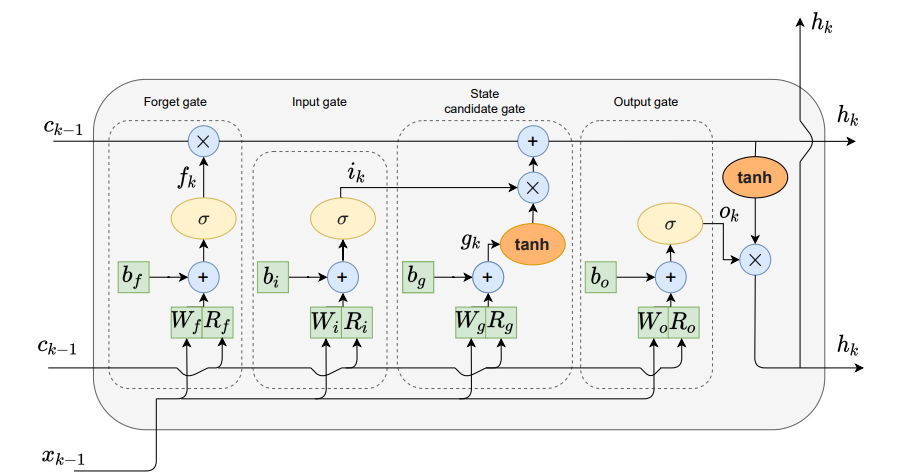
\includegraphics[width=0.75\linewidth]{Images/LSTM_Cell}
    \caption{Internal dataflow of an LSTM cell at time step $t$. The cell state
    $\mathbf{c}_t$ (horizontal channel) carries long-range memory; the forget gate
    $\mathbf{f}_t$, input gate $\mathbf{i}_t$, and output gate $\mathbf{o}_t$
    regulate what is erased, written, and read at each step. The hidden state
    $\mathbf{h}_t$ is derived from the cell state via the output gate.}
    \label{fig:lstm_cell}
    \end{figure}

    \noindent 
    The total parameter count for a single LSTM layer is $4(n_x d + d^2 + d)$, four times that of the basic RNN. This additional capacity improves the modelling of long-range dependencies but increases both memory requirements
    and training time substantially. The Gated Recurrent Unit, introduced in the following section, addresses this cost by merging the cell and hidden states into a single vector and replacing the four-gate mechanism with two gates, reducing the parameter count to $3(n_x d + d^2 + d)$ without significant loss in modelling performance \citep{chung2014empirical}. \\

    \section*{Gated Recurrent Units}

    The \textbf{Gated Recurrent Unit} (GRU) was introduced by \citet{cho2014learning} as a simplified gating architecture that mitigates the vanishing gradient problem whilst retaining fewer parameters than the Long Short-Term Memory network \citep{hochreiter1997long}. The GRU controls information flow through two learned gating vectors, an \textbf{update gate} $\mathbf{z}_t$ and a \textbf{reset gate} $\mathbf{r}_t$, both of which take values in $(0, 1)^d$ and operate element-wise on the hidden state. \\

    \noindent 
    At each time step $t$, given input $\mathbf{x}_t \in \mathbb{R}^{n_x}$ and previous hidden state $\mathbf{h}_{t-1} \in \mathbb{R}^d$, the GRU computes:

    \begin{align}
    \mathbf{z}_t &= \sigma\!\left(W_z\, \mathbf{x}_t
    + U_z\, \mathbf{h}_{t-1} + \mathbf{b}_z\right), \label{eq:gru_update} \\
    \mathbf{r}_t &= \sigma\!\left(W_r\, \mathbf{x}_t
    + U_r\, \mathbf{h}_{t-1} + \mathbf{b}_r\right), \label{eq:gru_reset} \\
    \tilde{\mathbf{h}}_t &= \tanh\!\left(W_h\, \mathbf{x}_t
    + U_h\,(\mathbf{r}_t \odot \mathbf{h}_{t-1}) + \mathbf{b}_h\right),
    \label{eq:gru_candidate} \\
    \mathbf{h}_t &= (1 - \mathbf{z}_t) \odot \mathbf{h}_{t-1}
    + \mathbf{z}_t \odot \tilde{\mathbf{h}}_t, \label{eq:gru_hidden}
    \end{align}

    \noindent 
    where $\sigma$ is the sigmoid function, $\odot$ denotes the Hadamard (element-wise) product, and $W_z, W_r, W_h \in \mathbb{R}^{n_x \times d}$ and $U_z, U_r, U_h \in \mathbb{R}^{d \times d}$ are learned parameter matrices. The
    computation in Equations~\eqref{eq:gru_update}--\eqref{eq:gru_hidden} admits the following interpretation. \\

    \noindent 
    The \textbf{update gate} $\mathbf{z}_t$ governs how much of the previous hidden state is preserved in the new hidden state. When $\mathbf{z}_t \approx \mathbf{0}$, the hidden state is carried forward unchanged from $\mathbf{h}_{t-1}$; when $\mathbf{z}_t \approx \mathbf{1}$, the hidden state is replaced entirely by the candidate $\tilde{\mathbf{h}}_t$. The network learns to open or close this gate adaptively based on the input and the current state. \\

    \noindent 
    The \textbf{reset gate} $\mathbf{r}_t$ controls how much of the previous hidden state is made available when computing the candidate $\tilde{\mathbf{h}}_t$. When $\mathbf{r}_t \approx \mathbf{0}$, the previous hidden state is suppressed and the candidate is computed as if from a fresh initialisation, allowing the network to discard accumulated context that is no longer relevant. When $\mathbf{r}_t \approx \mathbf{1}$, the full previous state is incorporated.\\

    \noindent 
    The \textbf{candidate hidden state} $\tilde{\mathbf{h}}_t$
    (Equation~\eqref{eq:gru_candidate}) is a $\tanh$-activated combination of the
    current input and the gated previous state. It represents the new information that
    could potentially enter the hidden state at this time step. \\

    \noindent 
    The \textbf{final hidden state} $\mathbf{h}_t$ (Equation~\eqref{eq:gru_hidden})
    is a convex interpolation between the previous hidden state and the candidate,
    with interpolation weights determined by the update gate. Crucially, this
    interpolation creates a near-direct path from $\mathbf{h}_{t-1}$ to $\mathbf{h}_t$
    whenever $\mathbf{z}_t$ is small. When unrolled across $T$ steps, this path
    prevents the gradient from vanishing: the derivative
    $\partial \mathbf{h}_t / \partial \mathbf{h}_{t-k}$ is no longer a product of
    $k$ Jacobians but instead accumulates additively, much as residual connections do
    in feedforward networks. This is the mechanism by which the GRU addresses the
    fundamental limitation of the basic RNN.

    The total number of learnable parameters in a single GRU layer with input dimension
    $n_x$ and hidden dimension $d$ is $3(n_x d + d^2 + d)$, corresponding to the three
    sets of weight matrices and bias vectors in Equations~\eqref{eq:gru_update},
    \eqref{eq:gru_reset}, and \eqref{eq:gru_candidate}. This is two-thirds the parameter
    count of an equivalent LSTM layer, which maintains both a hidden state and a separate
    cell state \citep{chung2014empirical}. Empirical comparisons indicate that the GRU
    matches LSTM performance on many sequence modelling tasks whilst being faster to
    train, a finding that motivates its use in the computationally intensive xVA context
    of this study \citep{chung2014empirical}.

    For a multi-layer GRU, the hidden state $\mathbf{h}_t^{(\ell)}$ at layer $\ell$
    takes the hidden state $\mathbf{h}_t^{(\ell-1)}$ from the layer below as its input
    $\mathbf{x}_t$, stacking the recurrent computation across depth. The output of the
    GRU at each time step $t$ is typically a linear function of the final-layer hidden
    state $\mathbf{h}_t^{(L)}$, and for sequence-to-one prediction tasks (such as
    predicting a scalar xVA quantity from a simulated path), the hidden state at the
    terminal time step $\mathbf{h}_T^{(L)}$ is passed to a feedforward output layer.

    \begin{figure}[htbp]
    \centering
    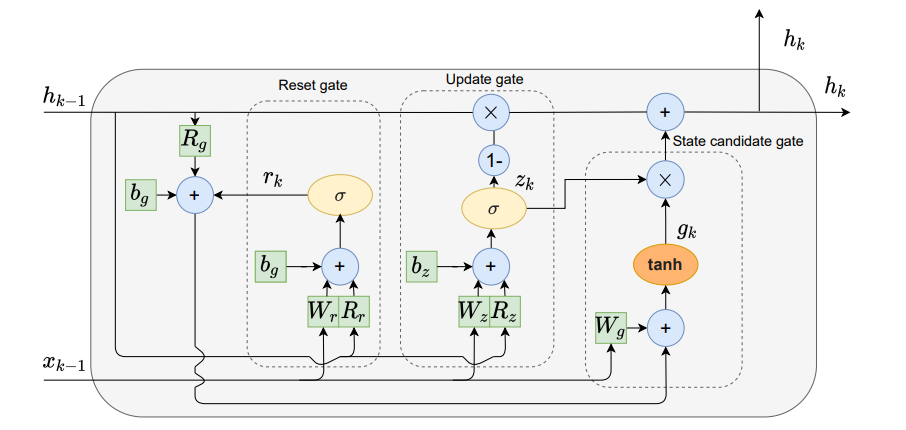
\includegraphics[width=0.75\linewidth]{Images/GRU_Cell}
    \caption{Internal dataflow of a GRU cell at time step $t$. The update gate
    $\mathbf{z}_t$ interpolates between the previous state $\mathbf{h}_{t-1}$
    (weighted by $1 - \mathbf{z}_t$) and the candidate $\tilde{\mathbf{h}}_t$
    (weighted by $\mathbf{z}_t$). The reset gate $\mathbf{r}_t$ controls how
    much of $\mathbf{h}_{t-1}$ enters the candidate computation. The near-direct
    path from $\mathbf{h}_{t-1}$ to $\mathbf{h}_t$ when $\mathbf{z}_t \approx 0$
    is the mechanism that prevents gradient vanishing across long sequences.}
    \label{fig:gru_cell}
    \end{figure}

    \section*{Optimisation}

    \subsection*{Gradient Descent Variants}

    Full-batch gradient descent computes the exact gradient of the loss over all $N$
    training samples before updating weights. This is computationally expensive per
    step and slow to converge when $N$ is large. \textbf{Stochastic gradient descent}
    (SGD) updates weights after every single training sample, approximating the
    gradient with a high-variance single-sample estimate. This is cheap per step but
    introduces substantial noise into the optimisation trajectory.

    \textbf{Mini-batch gradient descent} balances these extremes. Weights are updated
    after processing a mini-batch of $M$ samples, where $1 < M \ll N$. The averaged
    gradient

    \[
    \overline{g}_{w_{mn}} = \frac{1}{M} \sum_{i=1}^{M}
    \frac{\partial L^{(i)}}{\partial w_{mn}}\bigg|_\mathbf{W}
    \]

    is a lower-variance estimate than the single-sample SGD gradient, whilst updates
    remain frequent enough to exploit gradient information efficiently. Mini-batch
    training also maps naturally to GPU parallelism and is the standard approach
    in practice \citep{goodfellow2016deep}.

    \subsection*{Adaptive Learning Rate Methods}

    The Adam optimiser \citep{kingma2015adam} augments mini-batch gradient descent
    with adaptive per-parameter learning rates. Adam maintains exponentially decaying
    averages of past gradients (first moment $m_t$) and past squared gradients (second
    moment $v_t$):

    \begin{align*}
    m_t &= \beta_1 m_{t-1} + (1 - \beta_1)\, g_t, \\
    v_t &= \beta_2 v_{t-1} + (1 - \beta_2)\, g_t^2,
    \end{align*}

    with bias-corrected estimates $\hat{m}_t = m_t/(1 - \beta_1^t)$ and
    $\hat{v}_t = v_t/(1 - \beta_2^t)$. The parameter update is

    \[
    \theta_t = \theta_{t-1} - \frac{\eta}{\sqrt{\hat{v}_t} + \epsilon}\, \hat{m}_t,
    \]

    with standard defaults $\beta_1 = 0.9$, $\beta_2 = 0.999$, $\epsilon = 10^{-8}$
    \citep{kingma2015adam}. The second moment normalises the step size
    per-parameter: directions with consistently large gradients are taken with smaller
    effective learning rates, whilst directions with small or noisy gradients are
    amplified. Adam is robust across a wide range of architectures and is used as
    the default optimiser in this study.

    \section*{Regularisation and Generalisation}

    \subsection*{Overfitting and the Bias-Variance Tradeoff}

    A network trained to minimise training loss can memorise the training data,
    including noise, and perform poorly on previously unseen inputs. This is
    \textbf{overfitting}. The underlying tension is between bias and variance
    \citep{hastie2009elements}: a low-capacity model is biased toward simpler
    functions and may underfit (high training error regardless of data volume);
    a high-capacity model can represent complex functions but absorbs noise in
    the training data, producing high variance in predictions on new inputs.

    The standard diagnostic is to monitor training loss $L_T$ and validation loss
    $L_V$ across epochs. Both decrease initially as the network learns the underlying
    function. When $L_V$ begins to increase whilst $L_T$ continues to fall, the
    network is fitting noise. Training is stopped at the epoch of minimum $L_V$:
    this is \textbf{early stopping}, which uses the validation set as a proxy for
    generalisation performance.

    \subsection*{Weight Regularisation}

    Explicit regularisation modifies the loss function to penalise large weights,
    reducing the effective capacity of the network. The two standard forms are:

    \[
    L_2(\mathbf{y}, \mathbf{t}) = L(\mathbf{y}, \mathbf{t}) + \frac{\lambda}{2}
    \sum_{\text{all } w_{mn}} w_{mn}^2,
    \]

    \[
    L_1(\mathbf{y}, \mathbf{t}) = L(\mathbf{y}, \mathbf{t}) + \lambda
    \sum_{\text{all } w_{mn}} |w_{mn}|.
    \]

    Under $L_2$ regularisation, the modified weight update includes a shrinkage
    term proportional to the current weight:
    $w_{mn} \leftarrow w_{mn} - \eta(\partial L/\partial w_{mn}) - \eta\lambda w_{mn}$.
    This is called \textbf{weight decay}, and its effect is to pull all weights toward
    zero proportionally to their magnitude, preventing any single weight from
    becoming excessively large. Under $L_1$ regularisation, the update instead
    subtracts a constant-sign term:
    $w_{mn} \leftarrow w_{mn} - \eta(\partial L/\partial w_{mn}) - \eta\lambda
    \operatorname{sign}(w_{mn})$. The $L_1$ penalty drives small weights to exactly
    zero, producing sparse weight configurations. The regularisation coefficient
    $\lambda$ is a hyperparameter tuned using the validation set
    \citep{hastie2009elements}.

    \subsection*{Dataset Partitioning}

    Training a network that generalises requires discipline in how data is used.
    The dataset is partitioned into three disjoint subsets: the \textbf{training set},
    used to update weights; the \textbf{validation set}, used to monitor overfitting
    and tune hyperparameters; and the \textbf{test set}, used once at the conclusion
    of training to report final model performance. A typical partition is 50\% training,
    25\% validation, and 25\% test, with all subsets drawn randomly from the full
    dataset. Using the test set during model development invalidates its role as an
    unbiased estimator of generalisation error.

    When training data is limited, $k$-fold cross-validation provides more reliable
    generalisation estimates. The dataset is divided into $k$ equal folds and the
    training-testing procedure is repeated $k$ times, each time holding out a different
    fold. The performance metric is averaged over all $k$ rounds, and every data point
    is used for testing exactly once \citep{hastie2009elements}.

    \section*{Data Preparation}

    Neural network training is sensitive to the scale of input features. When features
    span very different numerical ranges, the contributions of different inputs to the
    pre-activation at the first hidden layer are unequal. Inputs with large magnitudes
    dominate the activation and drive the weight updates during early training, whilst
    the network is slow to resolve the influence of smaller-valued inputs. Normalising
    all features to a common scale before training reduces this problem and improves
    convergence.

    Two methods are standard. \textbf{Min-max normalisation} maps each feature to
    the interval $[0, 1]$:

    \[
    \tilde{d} = \frac{d - d_{\min}}{d_{\max} - d_{\min}}.
    \]

    \textbf{Z-score standardisation} rescales each feature to zero mean and unit
    variance:

    \[
    \tilde{d} = \frac{d - \mu}{\sigma},
    \]

    where $\mu$ and $\sigma$ are the sample mean and standard deviation computed from
    the training set. Both transformations are invertible, so predictions in the
    normalised space can be mapped back to original units. Z-score standardisation
    is generally preferred when the input distribution is not bounded and may be
    approximately Gaussian \citep{goodfellow2016deep}. In the context of this study,
    input features include short rates, time-to-maturity, and notionals, which span
    several orders of magnitude and are standardised prior to network training. Target
    prices are likewise normalised to improve numerical conditioning of the
    optimisation.

    \section*{Summary}

    This chapter has developed the theoretical machinery of neural networks and deep
    learning that underpins the surrogate pricing methodology of this study. Beginning
    with the artificial neuron and the perceptron learning rule, we have established how
    multi-layer architectures achieve non-linear function approximation. The Universal
    Approximation Theorem provides the existence guarantee that justifies applying
    neural networks to continuous pricing functions defined on compact domains.
    Backpropagation operationalises gradient descent by efficiently computing parameter
    gradients via the chain rule, with explicit delta formulas derived for MSE and
    cross-entropy losses.

    The feedforward MLP, whilst theoretically expressive, treats observations as
    independent. For pricing problems indexed by a simulation time grid, a recurrent
    architecture is more natural. The Gated Recurrent Unit addresses the vanishing
    gradient limitation of the basic RNN through an update gate and a reset gate, which
    create direct gradient pathways across time steps and allow the network to
    selectively retain or discard accumulated context. Mini-batch optimisation with
    Adam, combined with $L_2$ regularisation and early stopping, addresses the
    practical challenges of training on finite datasets. Data normalisation ensures
    numerical stability when inputs span disparate scales.

    With these foundations established, the following chapter presents the differential
    deep learning framework of \citet{mrad2025differential}, which augments the
    surrogate architecture with pathwise sensitivity information, enabling simultaneous
    approximation of prices and Greeks from a single trained network with substantially
    improved sample efficiency.

